\documentclass[pdf]{beamer}
\usetheme{default}
\graphicspath{ {imagenes/} }
\usepackage{graphicx}
\usepackage{eurosym}
\usepackage{subfig}
\newtheorem{prop}{Proposición}
\newtheorem{obv}{Observación}
\newtheorem{defi}{Definición}

%\mode<presentation>{\usetheme{Warsaw}}

\usepackage{pgfpages}
%\setbeameroption{show notes on second screen}

\usepackage[utf8]{inputenc}

\usepackage{graphicx}
\usepackage {mathtools}
\usepackage{utopia} %font utopia imported
\usetheme{Frankfurt}
\setbeamertemplate{footline}[frame number]

\usepackage{multicol}

\usepackage{tikz}
\usetikzlibrary{shapes.geometric, arrows}

% set colors

\usefonttheme{professionalfonts}
\usepackage{natbib}
\usepackage{hyperref}

%------------------------------------------------------------
%\titlegraphic{
\includegraphics[height=2cm]{logo.png}} 

\setbeamerfont{title}{size=\large}

\setbeamerfont{author}{size=\large}
\setbeamerfont{subtitle}{size=\small}
\setbeamerfont{date}{size=\small}
\setbeamerfont{institute}{size=\small}
\title{Sistemas de adaptación motora en entorno de realidad virtual}
\subtitle{ }  %% Change project title here
\author{Celia Arias Martínez } %% Change author name here
\setbeamerfont{page number in head/foot}{}

\institute{Tutores: Eduardo Ros Vidal y Jesús Garrido Alcázar\\
}
\date[\textcolor{white}{5 Julio 2023}]  %% Change presentation date here
{5 Julio 2023}

\logo{
	
\includegraphics[width=1cm]{ugr2.png}
}



\AtBeginSection[]
{
	  \begin{frame}
		    \frametitle{Contents}
		    \tableofcontents[currentsection]
		 \end{frame}
	}



%\title{Sistema de adaptación motora con entorno de realidad virtual}
%\author{Celia Arias Martínez}
\begin{document}
	
		\begin{frame}
		\titlepage
		\begin{figure}[htpb]
			\begin{center}
				
\includegraphics[width=0.25\linewidth]{ugr2}
			\end{center}
		\end{figure}
	\end{frame}






\begin{frame}{}
		\tableofcontents[sectionstyle=show,subsectionstyle=show/shaded/hide,subsubsectionstyle=show/shaded/hide]
\end{frame}


\section{Introducción}


\begin{frame}
	\frametitle{Estado del arte}
	\begin{itemize}
		\item Realidad virtual
		\begin{itemize}
			\item[-] Head Mounted Display o gafas de realidad virtual
			\item[-]Simuladores de vuelo
			\item[-] Dispositivos hápticos
		\end{itemize}
		\item Aprendizaje y control de movimientos
	\end{itemize}
\begin{figure}
	\centering
	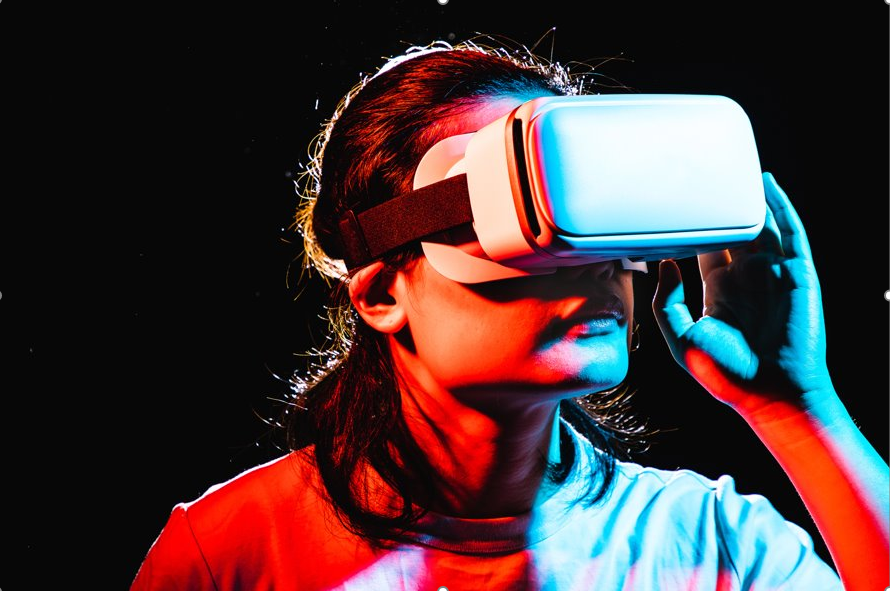
\includegraphics[width=0.65\textwidth]{virtual-reality}
\end{figure}
\end{frame}
\begin{frame}
	\frametitle{3D Systems Touch y OpenHaptics}
	
	\begin{figure}
		\centering
		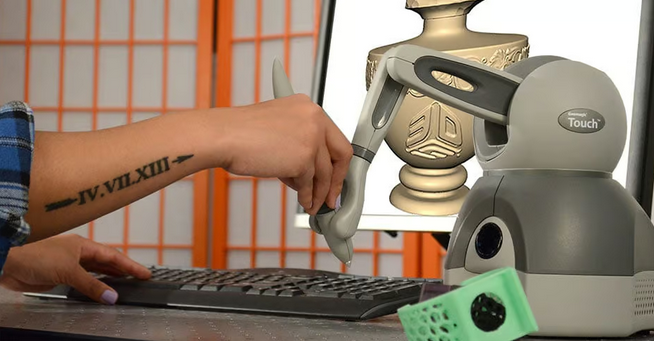
\includegraphics[width=0.6\textwidth]{touch}
	\end{figure}
	
	Dispositivo háptico desarrollado por \textbf{3D Systems} para simular objetos virtuales a medida que el usuario manipula objetos 3D en la pantalla.
	\begin{itemize}
		\item Control robótico
		\item Medicina y cirugía
		\item Rehabilitación.
	\end{itemize}		
\end{frame}
\begin{frame}
\frametitle{Objetivos}
\begin{itemize}
	\item Objetivos técnicos
	\begin{enumerate}
		\item Analizar cómo los dispositivos hápticos (en concreto \textit{3DSystems Touch}) pueden utilizarse en el estudio de movimientos balísticos.
		\item Estudiar la precisión de los datos obtenidos con el dispositivo \textit{Touch}.
		\item Interpretar dichos datos.
	\end{enumerate}
	\item Objetivos didáctivos
	\begin{enumerate}
		\item Aprender a usar \textit{3DSystems Touch}.
		\item Desarrollar una aplicación utilizando la API de \textit{Touch}.
		\item Entender algunas de las aplicaciones de la Geometría a la Informática Gráfica.
		\item Llevar a cabo una experimentación con diferentes sujetos.
		\item Realizar un análisis de los datos obtenidos.
	\end{enumerate}
\end{itemize}

\end{frame}

\begin{frame}
\frametitle{Fases del proyecto}	
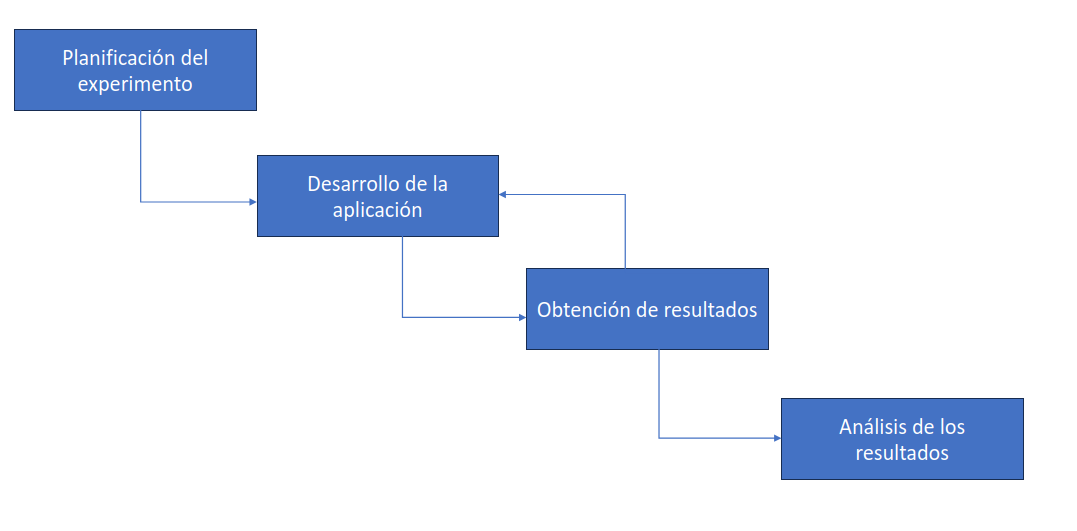
\includegraphics[width=\linewidth]{diagrama-fases}
\begin{itemize}
	\item Modelo de ciclo de vida en \textbf{cascada con realimentación}
\end{itemize}

\end{frame}




\section{Fundamentos matemáticos}
\begin{frame}
	\frametitle{¿Cómo obtenemos las coordenadas de las trayectorias que realizamos con el dispositivo Touch?}

		\begin{figure}
		\centering
		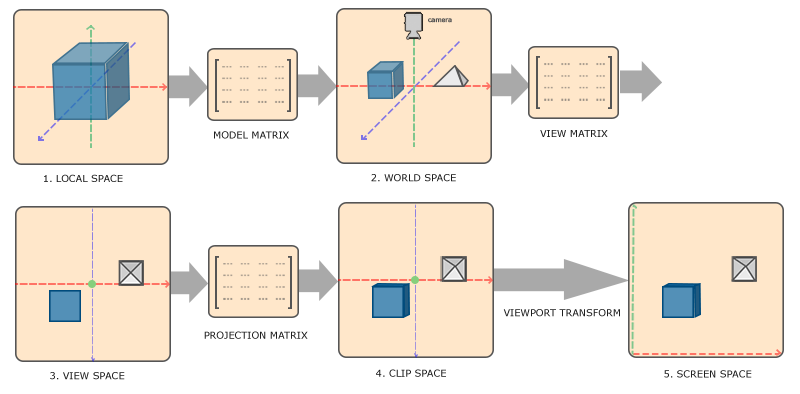
\includegraphics[width=\textwidth]{coordinate_systems}
	\end{figure}
\begin{itemize}
	\fontsize{10pt}{9pt}\selectfont
	\item Queremos transformar las coordenadas de pantalla a un sistema más intuitivo.
\end{itemize}
\end{frame}
\begin{frame}
	\frametitle{Tipos de transformaciones: Álgebra lineal}
	
	\begin{itemize}
		
		\item Escalados
		
	\end{itemize}

\begin{prop}
	\label{prop:cambio_base}
	Supongamos $V$ un espacio vectorial sobre un cuerpo $K$ con $dim_k(V) = n$. Tomamos dos bases $B = \{v_1,...,v_n\}$ y $B' = \{v_1',...,v_n'\}$ de $V$ y $ v \in V$ y sea $M(I, B' \leftarrow B)$ la matriz de cambio de base.
	\begin{equation}
		v_{B'} = M(I, B' \leftarrow B)\cdot  v_B
	\end{equation}
\end{prop}
\end{frame}
\begin{frame}
	\frametitle{Tipos de transformaciones: Espacio afín}
		\begin{itemize}
		\item Traslaciones
	\end{itemize}
	\begin{prop}
		Sea $R = \{p_0,...,p_n\} \equiv \{p_0, B\}$, $R' = \{p_0',...,p_n'\} \equiv \{p_0', B'\}$ y $M(Id_{\overrightarrow{A}}, B, B')$ la matriz de cambio de base de $B$ a $B'$. La fórmula del cambio de sistema de referencia es:
		\begin{equation}
			p_{R'} = (p_0)_{R'} + M(Id_{\overrightarrow{A}}, B, B')p_R
		\end{equation}
	\end{prop}
\begin{obv}
	Podemos escribir la fórmula anterior de la siguiente forma:
	\begin{equation}\label{cambio}
		\begin{pmatrix}
			1 \\
			p_{R'}
		\end{pmatrix}
		= \begin{pmatrix}
			M(Id, B, B') & (p_0)_{R'} \\
			0 			 & 1 \\
		\end{pmatrix}\cdot \begin{pmatrix}
			1 \\
			p_R
		\end{pmatrix}
	\end{equation}
\end{obv}
\end{frame}
\begin{frame}
	\frametitle{Tipos de transformaciones: Espacio proyectivo}
	\begin{itemize}
		\item Proyecciones
	\end{itemize}
	\begin{defi}
		Definiendo el hiperplano $A \subseteq \mathbb R^{n+1}$ donde $\{x_0 = 1\}$ como:
		\begin{equation}
			A = \{1\} \times \mathbb R^n \subseteq \mathbb R^{n+1}
		\end{equation}
	el embebimiento canónico de $\mathbb R^n$ en $\mathbb P^n$ será:
	Sea \begin{equation}
		e: \mathbb R^n \rightarrow A \textup{,   } e((x_1,...,x_n)) = (1:x_1:...:x_n)
	\end{equation}
	\end{defi}

	\begin{prop}
	La relación entre el espacio euclidiano $\mathbb R^n$ y el proyectivo $\mathbb P^n$ es:
\begin{equation}\label{cambio_proyectivo}
	\mathbb P^n \setminus \mathbb R^n_{\infty} \textup{ }   \underrightarrow{e^{-1}} \textup{ }\mathbb R^n \textup{,     } (x_0:x_1:...:x_n) \longmapsto (\frac{x_1}{x_0},...,\frac{x_n}{x_0})
\end{equation}


	\end{prop}
\end{frame}
\begin{frame}
\tikzstyle{process} = [rectangle, 
minimum width=3cm, 
minimum height=1cm, 
text centered, 
text width=3cm, 
draw=black, 
fill=orange!30]
\tikzstyle{arrow} = [thick,->,>=stealth]
\begin{center}
\begin{tikzpicture}[node distance=1cm]
	
	\node (start) [process, yshift=-0.5cm] {Coordenadas locales};
	\node (in1) [process, below of=start, yshift=-0.5cm] {Coordenadas de vista};
	\node (pro1) [process, below of=in1, yshift=-0.5cm] {Coordenadas de recorte};
	\node (dec1) [process, below of=pro1, yshift=-0.5cm] {Coordenadas de pantalla};
	
	\node (pro2a) [process, below of=dec1, yshift=-0.5cm] {Coordenadas finales};
	

	
	\draw [arrow] (start) -- (in1);
	\draw [arrow] (in1) -- (pro1);
	\draw [arrow] (pro1) -- (dec1);
	\draw [arrow] (dec1) --  (pro2a);
	
\end{tikzpicture}
\end{center}
	
\end{frame}
\begin{frame}
	\frametitle{Matriz modelview: C. Locales a C. Vista}


$$\textup{Matriz modelview}  := \begin{pmatrix}
	1 & 0 & 0& 0 \\
	0 & 1&0&0 \\
	0&0&1&-6.49 \\
	0&0&0&1
\end{pmatrix} = (Id, R', R)$$
\begin{block}{}

\begin{equation}
	p_{R'} = 
	\begin{pmatrix}
		0\\
		0\\
		-6.49
	\end{pmatrix}
	+
	\begin{pmatrix}
		1&0&0 \\
		0&1&0\\
		0&0&1
	\end{pmatrix}
	\cdot p_R
\end{equation}
\end{block}
\begin{itemize}
	\item \textbf{Traslación en el eje z}.
\end{itemize}
\end{frame}



\begin{frame}
	\frametitle{Matriz de proyección I: C. Vista a C. Recorte}
	\begin{columns}
		\column{.5\textwidth}
		\begin{figure}
			\centering
			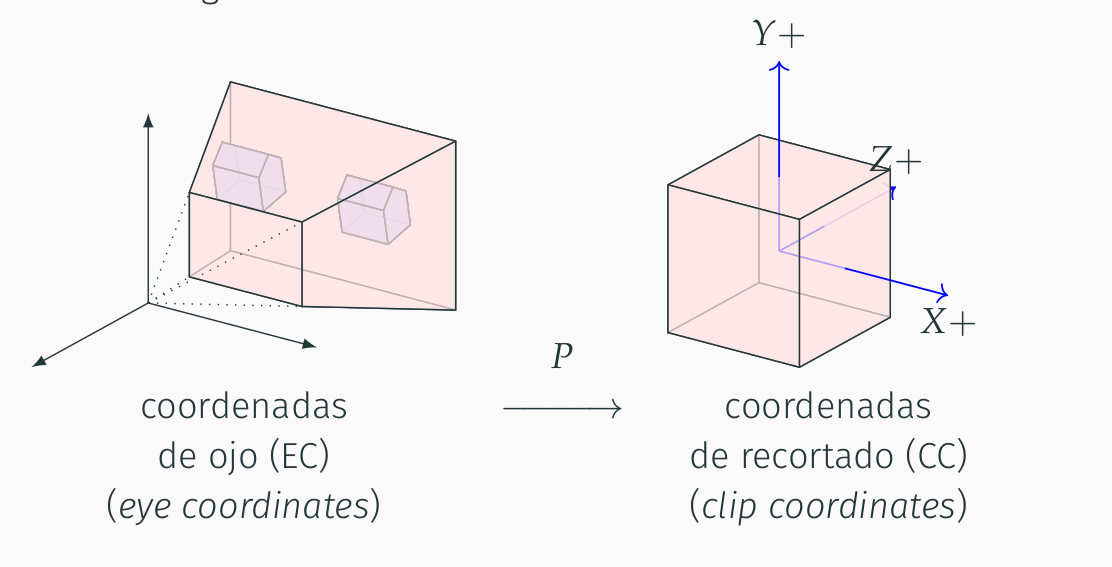
\includegraphics[width=\textwidth]{cubo}
		\end{figure}
	
		\column{.5\textwidth}
			\begin{figure}
			\centering
			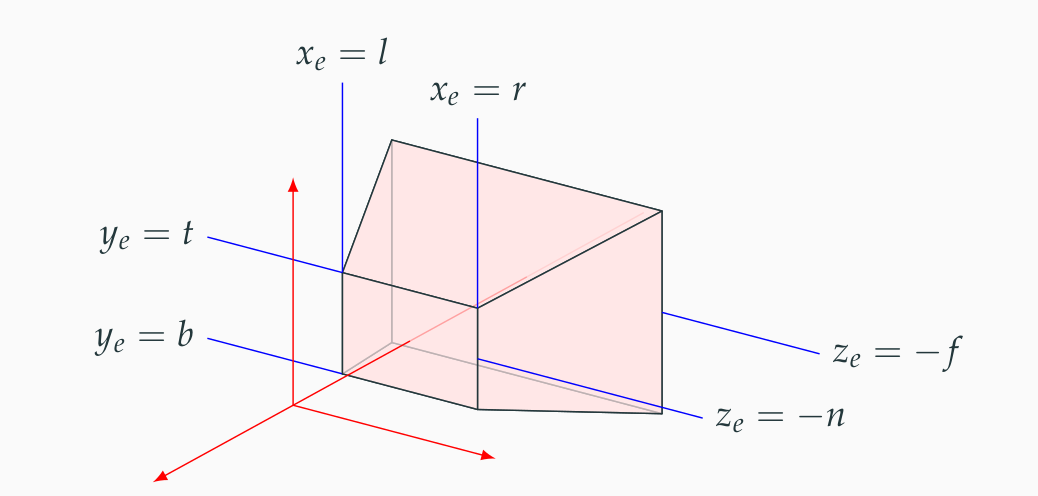
\includegraphics[width=\textwidth]{notacion}
		\end{figure}
	\end{columns}
	\begin{multicols}{2}
		
		\begin{enumerate}
		
			\item Proyección de $x,y$ sobre $z = -n$.
			\begin{equation*}
				x''_e = x'\cdot\frac{-n}{z'}
			\end{equation*}
			\begin{equation*}
				y''_e = y'\cdot\frac{-n}{z'}
			\end{equation*}
			\begin{equation*}
				z''_e = z'\cdot\frac{-n}{z'} = -n
			\end{equation*}
	
			\item Escalado y traslación de $x,y$ para llevarlos a $[-1,1]$.
			\begin{equation*}
				x'' =  \frac{a_0 \cdot x'+a_1 \cdot z'}{-z'}
			\end{equation*}
			\begin{equation*}
				y'' =  \frac{b_0 \cdot y'+b_1 \cdot z'}{-z'}
			\end{equation*}
		\end{enumerate}
	\end{multicols}
\end{frame}

\begin{frame}[t]
	\frametitle{Matriz de proyección II: C. Vista a C. Recorte}
	\begin{columns}
		\begin{column}{0.5\textwidth}
			\begin{enumerate}\setcounter{enumi}{2}
				\item Eliminación de partes ocultas
				\begin{equation*}
					z'' = \frac{c_0\cdot z'+c_1}{-z'}
				\end{equation*}
			\end{enumerate}
		\end{column}
		\begin{column}{0.5\textwidth}
		\begin{enumerate}\setcounter{enumi}{3}
		\item Guardamos el término no lineal.
		\begin{equation*}
			x'' = a_0 \cdot x'+a_1 \cdot z'
		\end{equation*}
		\begin{equation*}
			y'' = b_0 \cdot y'+b_1 \cdot z'
		\end{equation*}
		\begin{equation*}
			z'' = c_0\cdot z'+c_1
		\end{equation*}
		\begin{equation*}
			w'' = -z'
		\end{equation*}

	\end{enumerate}
\end{column}
\end{columns}
\begin{columns}
	\begin{column}{0.56\textwidth}
	\begin{block}{}
	$$\begin{pmatrix}
		x''\\
		y''\\
		z'' \\
		w
	\end{pmatrix}=
	\begin{pmatrix}
		a_0 & 0&a_1&0\\
		0&b_0&b_1&0\\
		0&0&c_0&c_1\\
		0&0&-1&0
	\end{pmatrix}\cdot 
	\begin{pmatrix}
		x'\\
		y'\\
		z'\\
		1
	\end{pmatrix}
	$$
\end{block}
\end{column}
\begin{column}{0.5\textwidth}
	\begin{block}{}
	$$\begin{pmatrix}
		2.74 & 0&0&0\\
		0&2.74 &0&0\\
		0&0&-3.74&-22.6\\
		0&0&-1&0
	\end{pmatrix}$$
	\end{block}
\end{column}

\end{columns}
\end{frame}

\begin{frame}
	\frametitle{Viewport: C. Recorte a C. Pantalla}
	\begin{columns}
		\begin{column}{0.5\textwidth}
		\begin{figure}
		\centering
		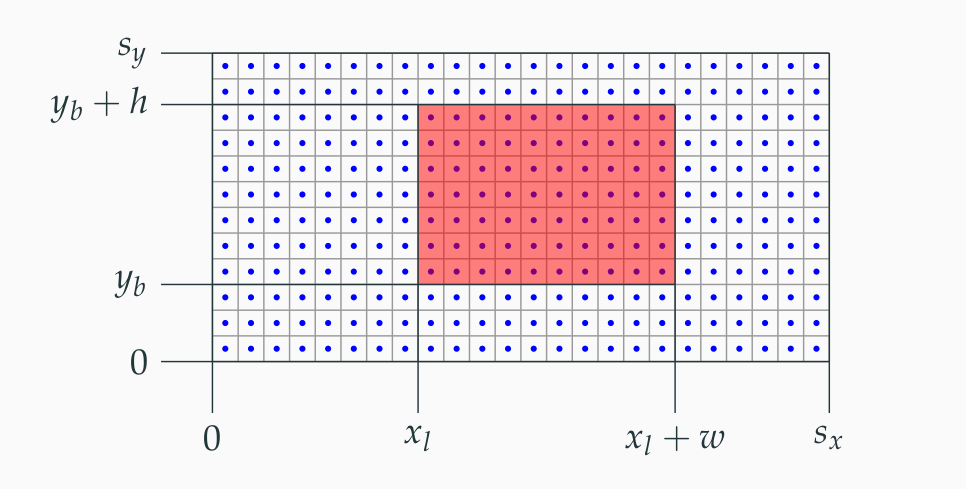
\includegraphics[width=\textwidth]{viewport}
	\end{figure}
\begin{equation*}
	x''' = (x''+1)\cdot \frac{w}{2}+a
\end{equation*}
\begin{equation*}
	y''' = (y''+1)\cdot \frac{h}{2}+b
\end{equation*}
\begin{equation*}
	z''' = (z''+1)\cdot \frac{f-n}{2}+n
\end{equation*}
			
	\end{column}
\begin{column}{0.5\textwidth}
	\begin{itemize}
		\item Eje $x$ al intervalo $[x_l, x_l+w]$.
		\item Eje $y$ al intervalo $[y_b, y_b+h]$.
		\item Eje $z$ al intervalo $[n, f]$.
		
	\end{itemize}
\begin{block}{}


$$\begin{pmatrix}
	\frac{w}{2} &0&0&\frac{w}{2}+a\\
	0&\frac{h}{2} &0&\frac{h}{2}+b\\
	0&0&\frac{f-n}{2} & \frac{f+n}{2}\\
	0&0&0&1
\end{pmatrix}$$

\begin{itemize}
	\item Escalado $[\frac{w}{2}, \frac{h}{2}, \frac{f-n}{2}]$ 
	\item Traslación $[\frac{w}{2}+a, \frac{h}{2}+b, \frac{f+n}{2}]$
\end{itemize}
\end{block}
\end{column}
\end{columns}


\end{frame}

\begin{frame}
	\frametitle{C. Pantalla a C. Finales}
	\begin{itemize}
		\item El punto $(0,0)$ de las coordenadas del dispositivo queremos llevarlo al origen. Por tanto calculamos las coordenadas de pantalla de dicho punto ($(250,250)$) y hacemos una traslación:
			\begin{equation*}
			x^{\romannumeral 4} = x'''-250
		\end{equation*}
		\begin{equation*}
			y^{\romannumeral 4} = y'''-250
		\end{equation*}
		\item Queremos que los targets estén en la circunferencia de radio $2$ y centro el punto de referencia. Hacemos un escalado, con 0.00945962 como factor de escala.
		 
	\end{itemize}
Por tanto tenemos:
\begin{block}{}
\begin{equation*}
	\begin{pmatrix}
		x^{\romannumeral 4}\\
		y^{\romannumeral 4}\\
		1
	\end{pmatrix} =
	\begin{pmatrix}
		0.0009 &0&-250\\
		0&0.0009&-250\\
		0&0&1 \\
	\end{pmatrix}
	\cdot \begin{pmatrix}
		x'''\\
		y'''\\
		1
	\end{pmatrix}
\end{equation*}
\end{block}
\end{frame}
\section{Implementación del proyecto}

\begin{frame}
	\frametitle{Tareas a realizar}

	\begin{enumerate}
		\item Situar el cursor sobre el punto de referencia (en el centro).
		\item Desaparece el punto de referencia y aparece otro punto situado en una de las 8 posiciones de la imagen (punto objetivo). 
		\item Al situar el cursor sobre el punto objetivo (o al acabarse el tiempo) el punto desaparece y vuelve a aparecer el punto de referencia.
	\end{enumerate}
\begin{columns}
	\begin{column}{0.5\textwidth}
	\begin{figure}
	\centering
	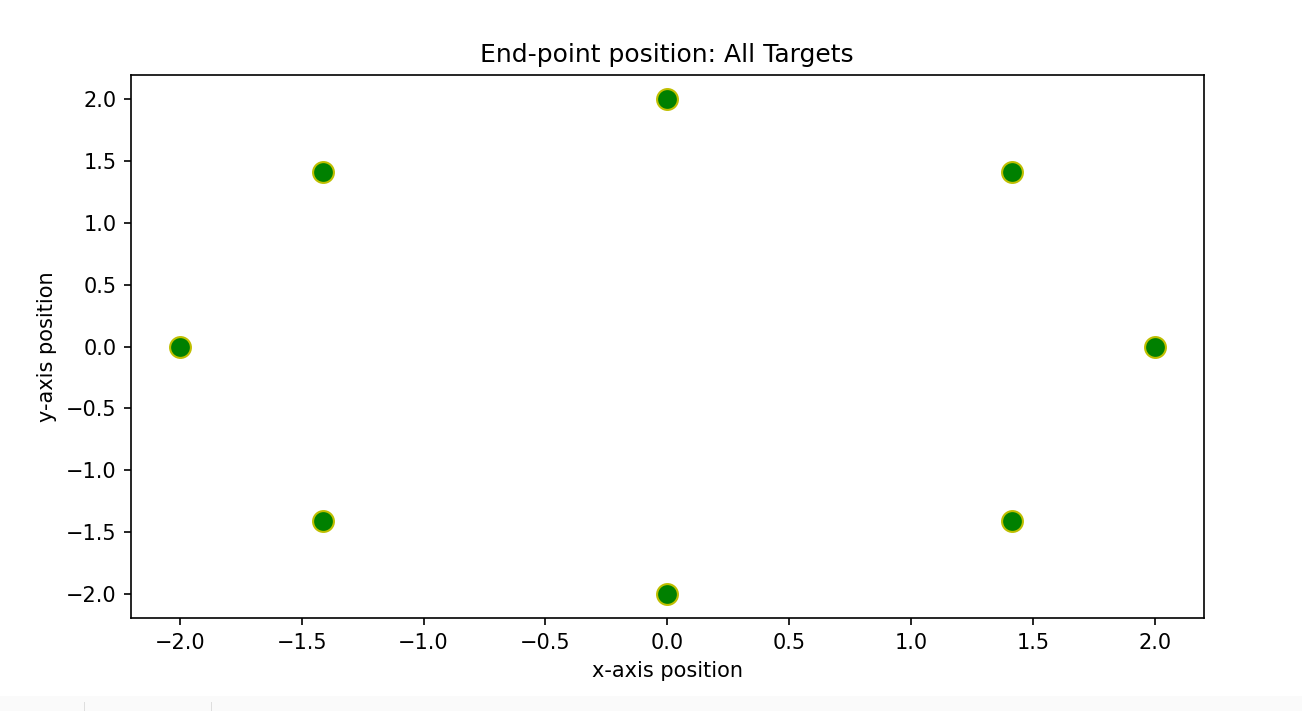
\includegraphics[width=\textwidth]{points}
\end{figure}	
\end{column}
\begin{column}{0.5\textwidth}
\begin{block}{}
	{\small Las trayectorias que guardaremos serán las del punto de referencia al punto objetivo.}
\end{block}	
\end{column}
\end{columns}

\end{frame}

\begin{frame}
	\frametitle{Fases del experimento}

	\begin{enumerate}
		\item \textbf{Fase libre}: no hay ningún target y el sujeto es libre de mover el cursor como quiera. 
		\item \textbf{Primera fase}: sin ninguna fuerza y mostrando el cursor.
		\item \textbf{Segunda fase}: con fuerza (en el eje x, sentido negativo) y mostrando el cursor.
		\item \textbf{Tercera fase}: sin fuerza y sin mostrar el cursor.
		\item \textbf{Cuarta fase}: con fuerza y sin mostrar el cursor.
	\end{enumerate}	
	\begin{itemize}
		\item En cada una de las fases se harán 80 repeticiones de la tarea definida antes.
	\end{itemize}
\end{frame}



\begin{frame}
	\frametitle{Desarrollo}
	\begin{columns}
		\begin{column}{0.4\textwidth}
				\begin{itemize}
				\item Bucle gráfico: 30 Hz.
				\item Servoloop: 1000 Hz, máxima prioridad.
			\end{itemize}
		\end{column}
		\begin{column}{0.6\textwidth}
			\textbf{Callbacks:}
			\begin{itemize}
				\item Síncronas o asíncronas
				\item Return code \textit{Done} o \textit{Continue}
			\end{itemize}
		\end{column}
	\end{columns}
	
	\begin{figure}
	\centering
	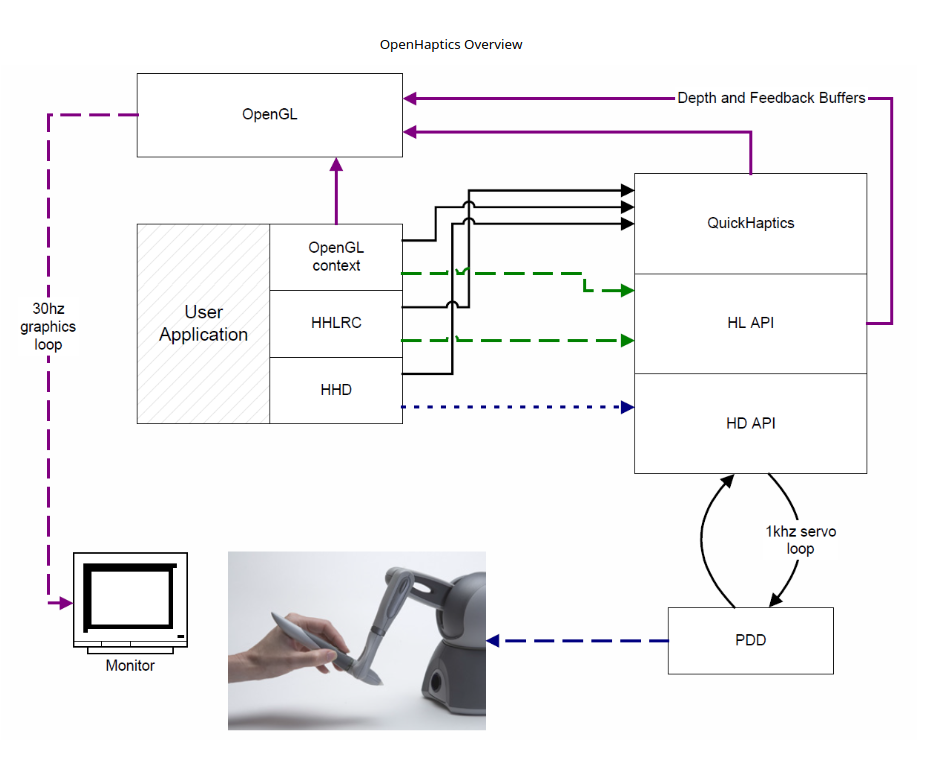
\includegraphics[width=0.7\textwidth]{estructura}
	\end{figure}

\end{frame}


\section{Resultados}

\begin{frame}
	\frametitle{Muestra de sujetos elegidos}
\begin{columns}
	\begin{column}{0.5\textwidth}
		\begin{table}[H]
			\centering
			\begin{tabular}{l l | l l}
				\multicolumn{2}{ c }{\textbf{Fase de prueba}} & \multicolumn{2}{ c }{\textbf{Fase final}} \\ 
				Sexo & Edad & Sexo & Edad\\\hline 
				
				Mujer & 23 & Mujer & 20 \\
				Mujer & 24  & Mujer & 22\\
				Hombre & 53 & Hombre & 50\\
				Mujer & 52 & Hombre & 60 \\
				Hombre & 62 & Mujer & 60\\
				Mujer & 60 \\
				Hombre & 90 \\
				Mujer & 90 \\
			\end{tabular} 
		\end{table}
	\end{column}

\begin{column}{0.35\textwidth}
	\begin{block}{}
	Parámetros elegidos en la fase de prueba:
	\begin{itemize}
		\item Nº de repeticiones
		\item Tiempo
		\item Nº y disposición de los targets
	\end{itemize}
\end{block}
\end{column}

\end{columns}

	
\end{frame}
\begin{frame}
	\frametitle{Nomenclatura de los sujetos}
\begin{columns}
	\begin{column}{0.5\textwidth}
		\begin{itemize}
			\item Sujeto 1: Mujer, 20 años, en orden
			\item Sujeto 2: Mujer, 22 años, aleatorio
			\item Sujeto 3: Mujer, 60 años, aleatorio
			\item Sujeto 4: Hombre, 50 años, en orden
			\item Sujeto 5: Hombre, 60 años, en orden
		\end{itemize}
	\end{column}
	\begin{column}{0.5\textwidth}
		\begin{figure}
			\centering
			
			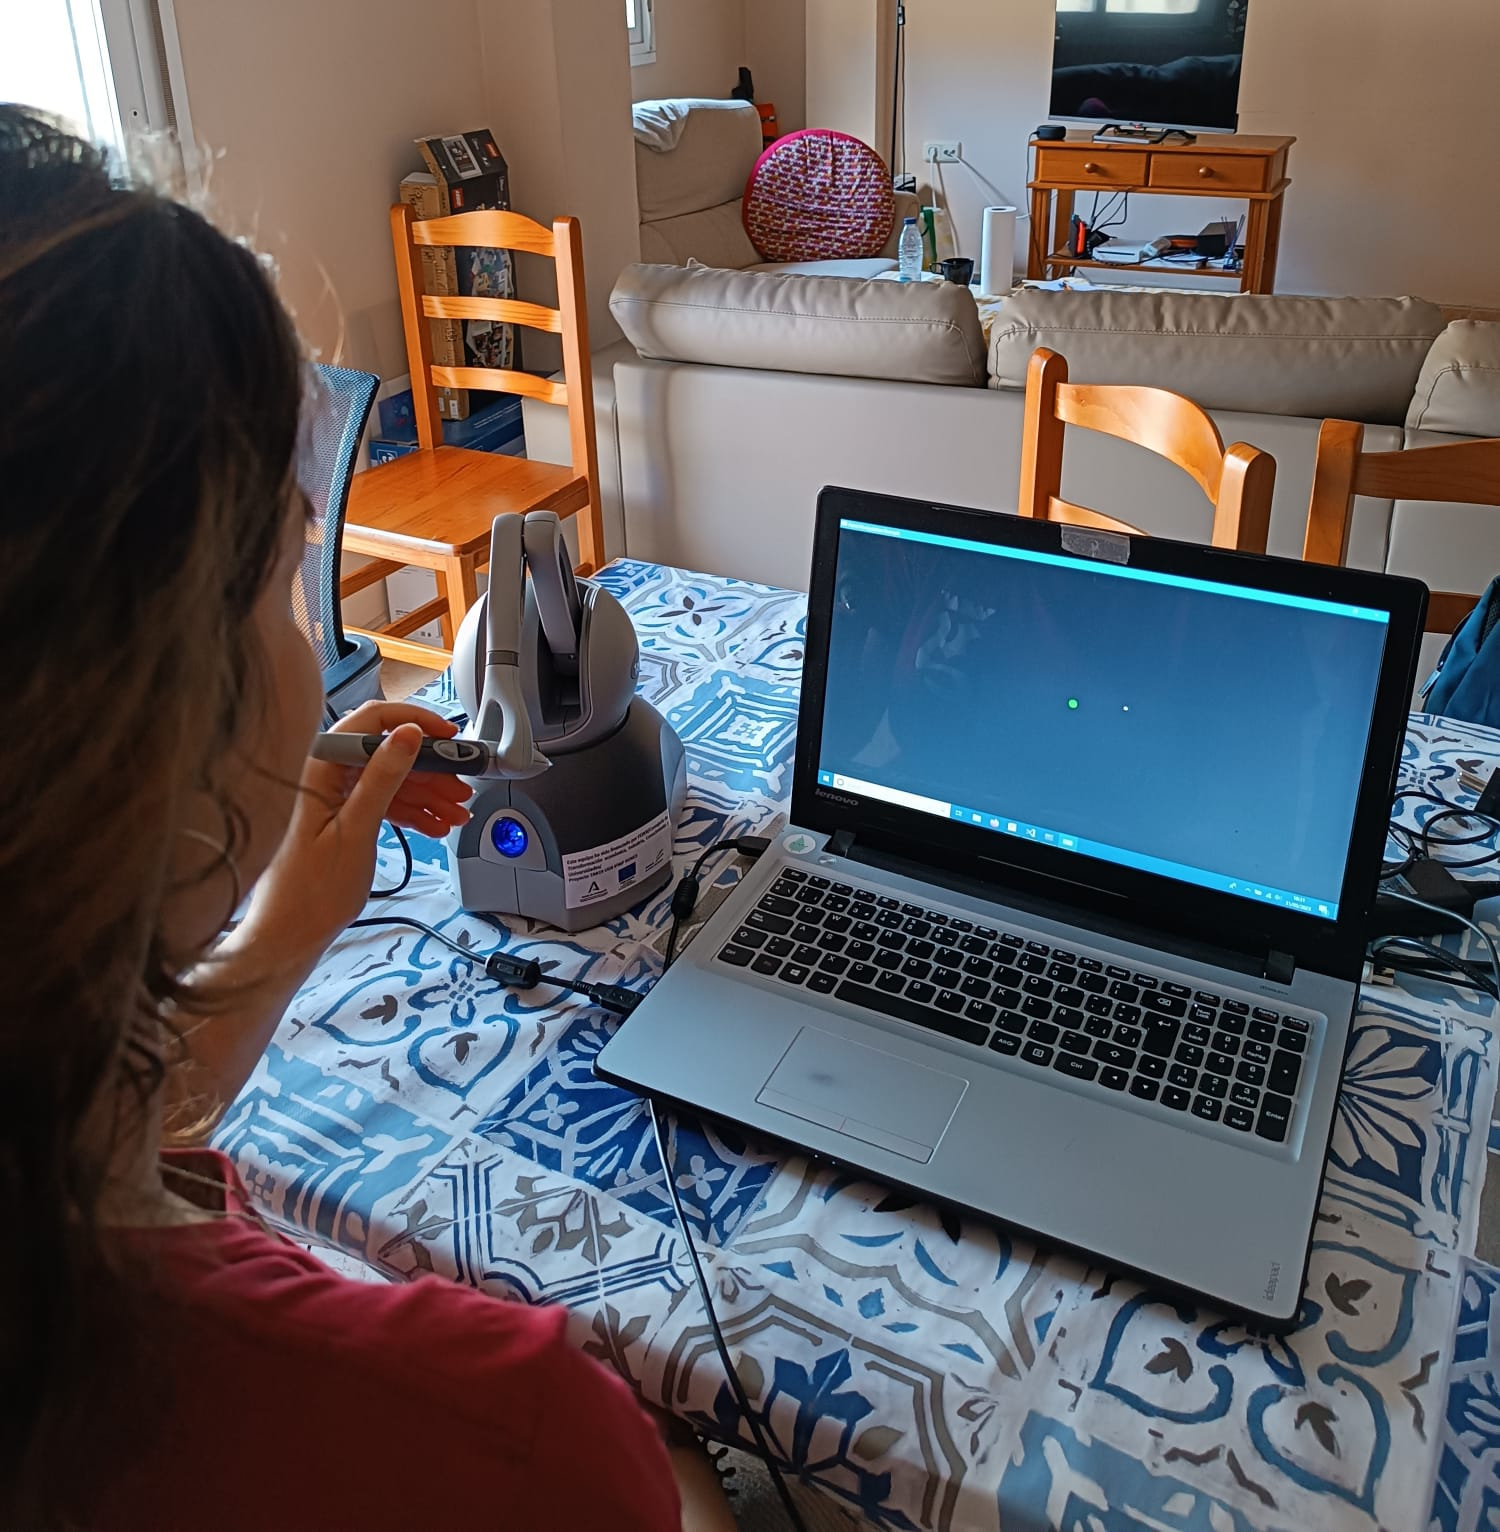
\includegraphics[width=\textwidth]{sujeto-2}
			
		\end{figure}
	\end{column}
\end{columns}
		

			
\end{frame}
\begin{frame}
	\frametitle{Aplicación}
	\begin{columns}
		\begin{column}{0.65\textwidth}
				\begin{figure}
				\centering
				
				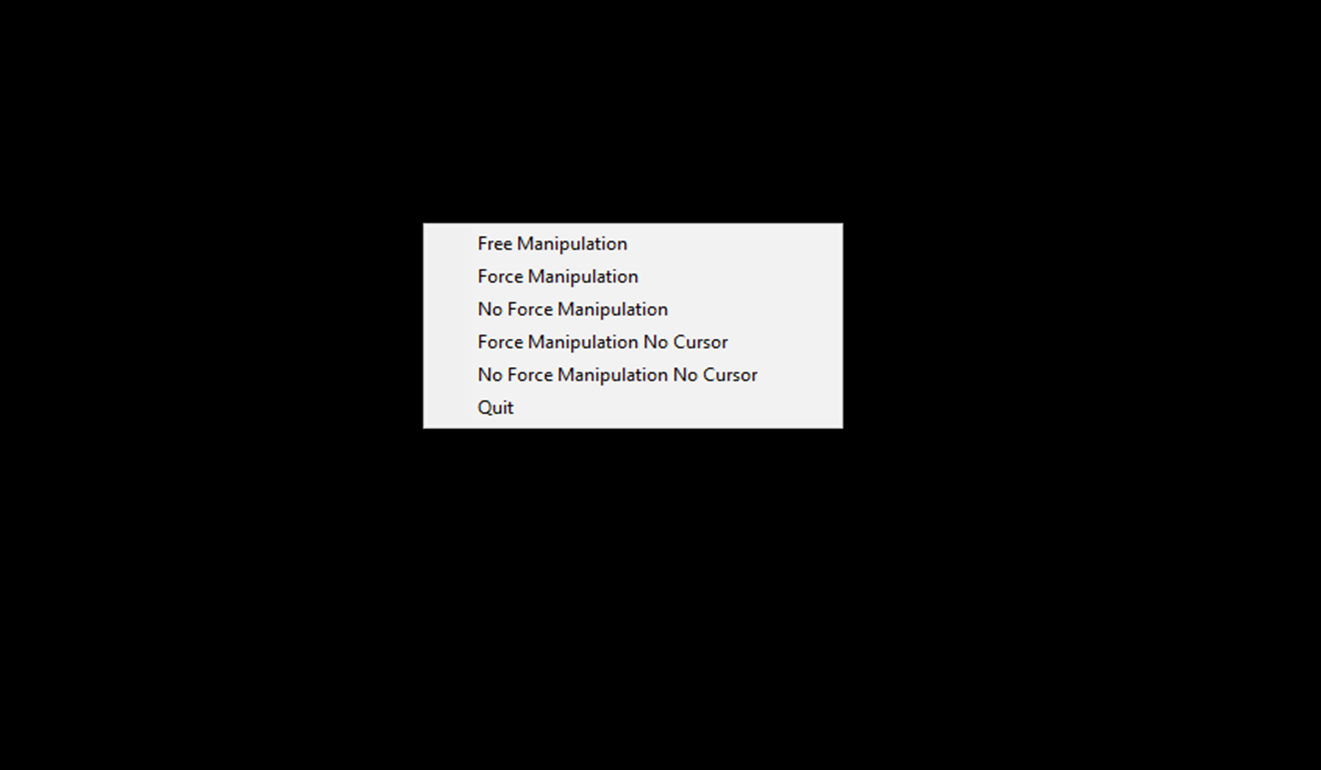
\includegraphics[width=\textwidth]{menu}
				
			\end{figure}
		\end{column}
	\begin{column}{0.35\textwidth}
	\begin{figure}
		\centering
		
		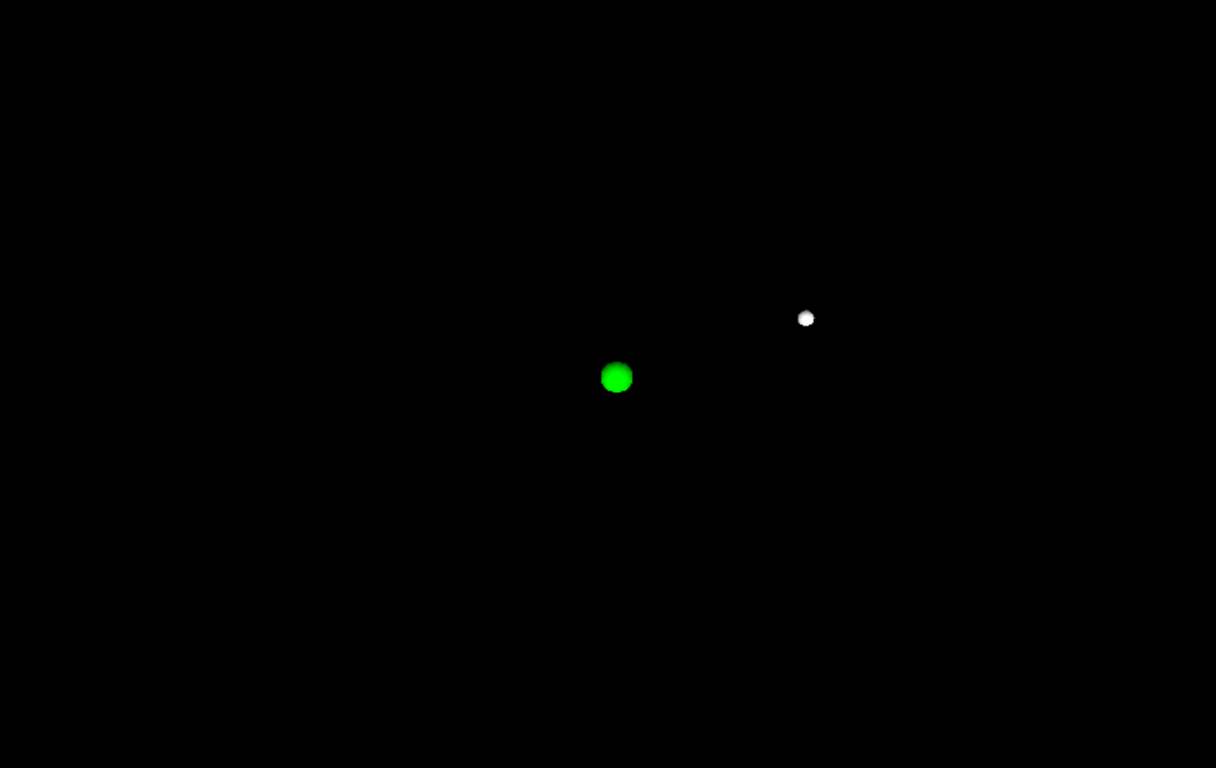
\includegraphics[width=\textwidth]{cursor}
		
	\end{figure}
	\end{column}
	\end{columns}
	

\end{frame}




\begin{frame}
	\frametitle{Fase 1: sin fuerza}
			\begin{itemize}
		\item Los sujetos jóvenes tienen más precisión y son más rápidos.
		\item El sujeto 5 muestra una curva de aprendizaje, el 3 no.
	\end{itemize}
	\begin{columns}
		\begin{column}{0.4\textwidth}
			\begin{figure}
			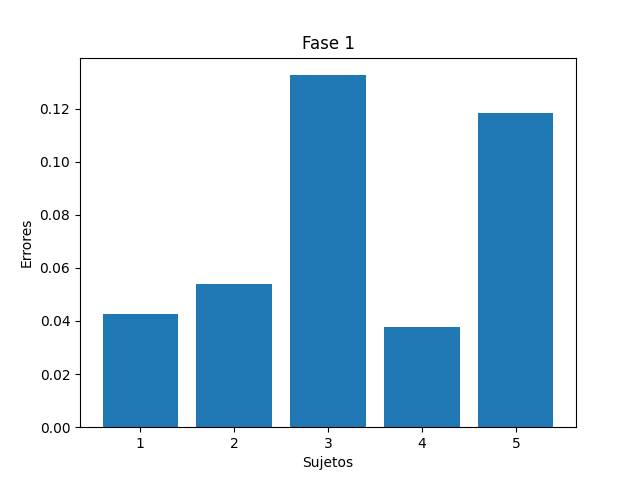
\includegraphics[width=\textwidth]{fase1-errores}
			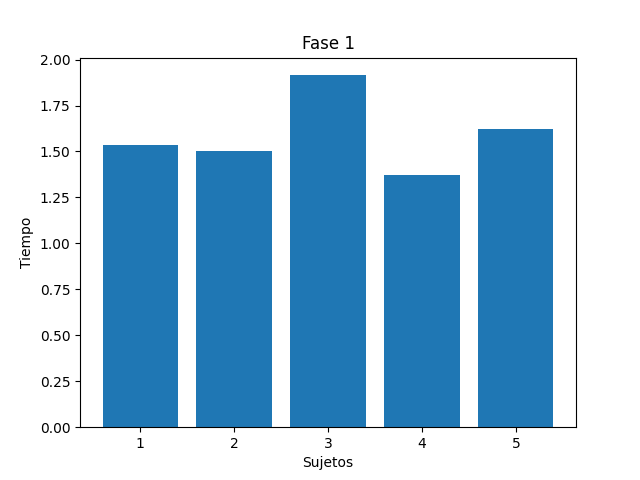
\includegraphics[width=\textwidth]{fase1-time}
			\end{figure}

		\end{column}
	\begin{column}{0.6\textwidth}
		\begin{figure}
			\centering
				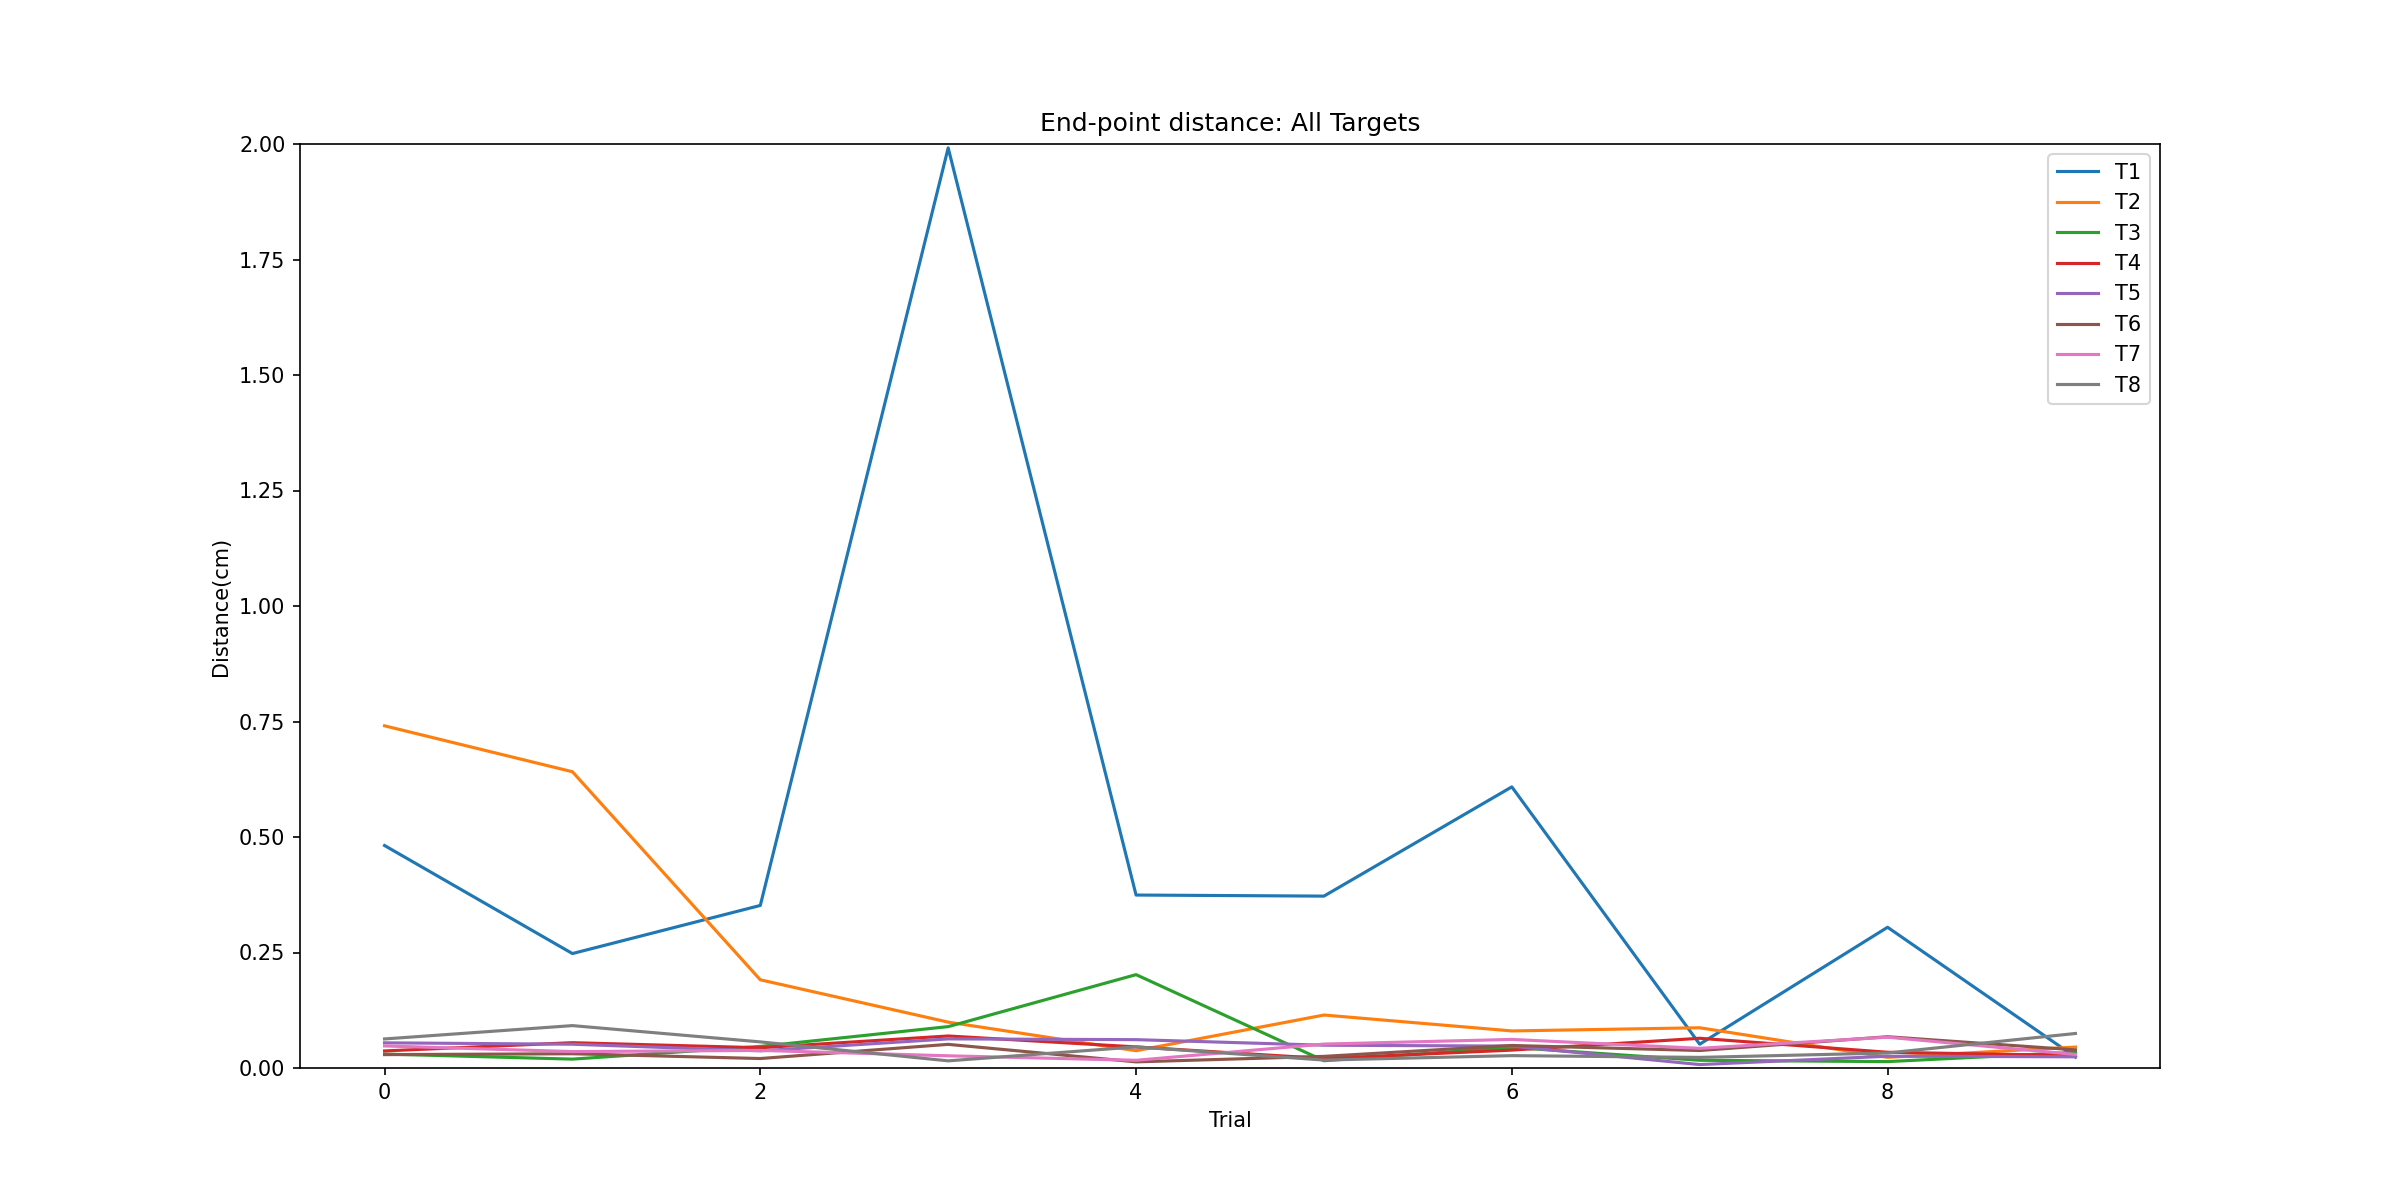
\includegraphics[width=\textwidth]{sujeto5/no_force/evolution_distance}
	
				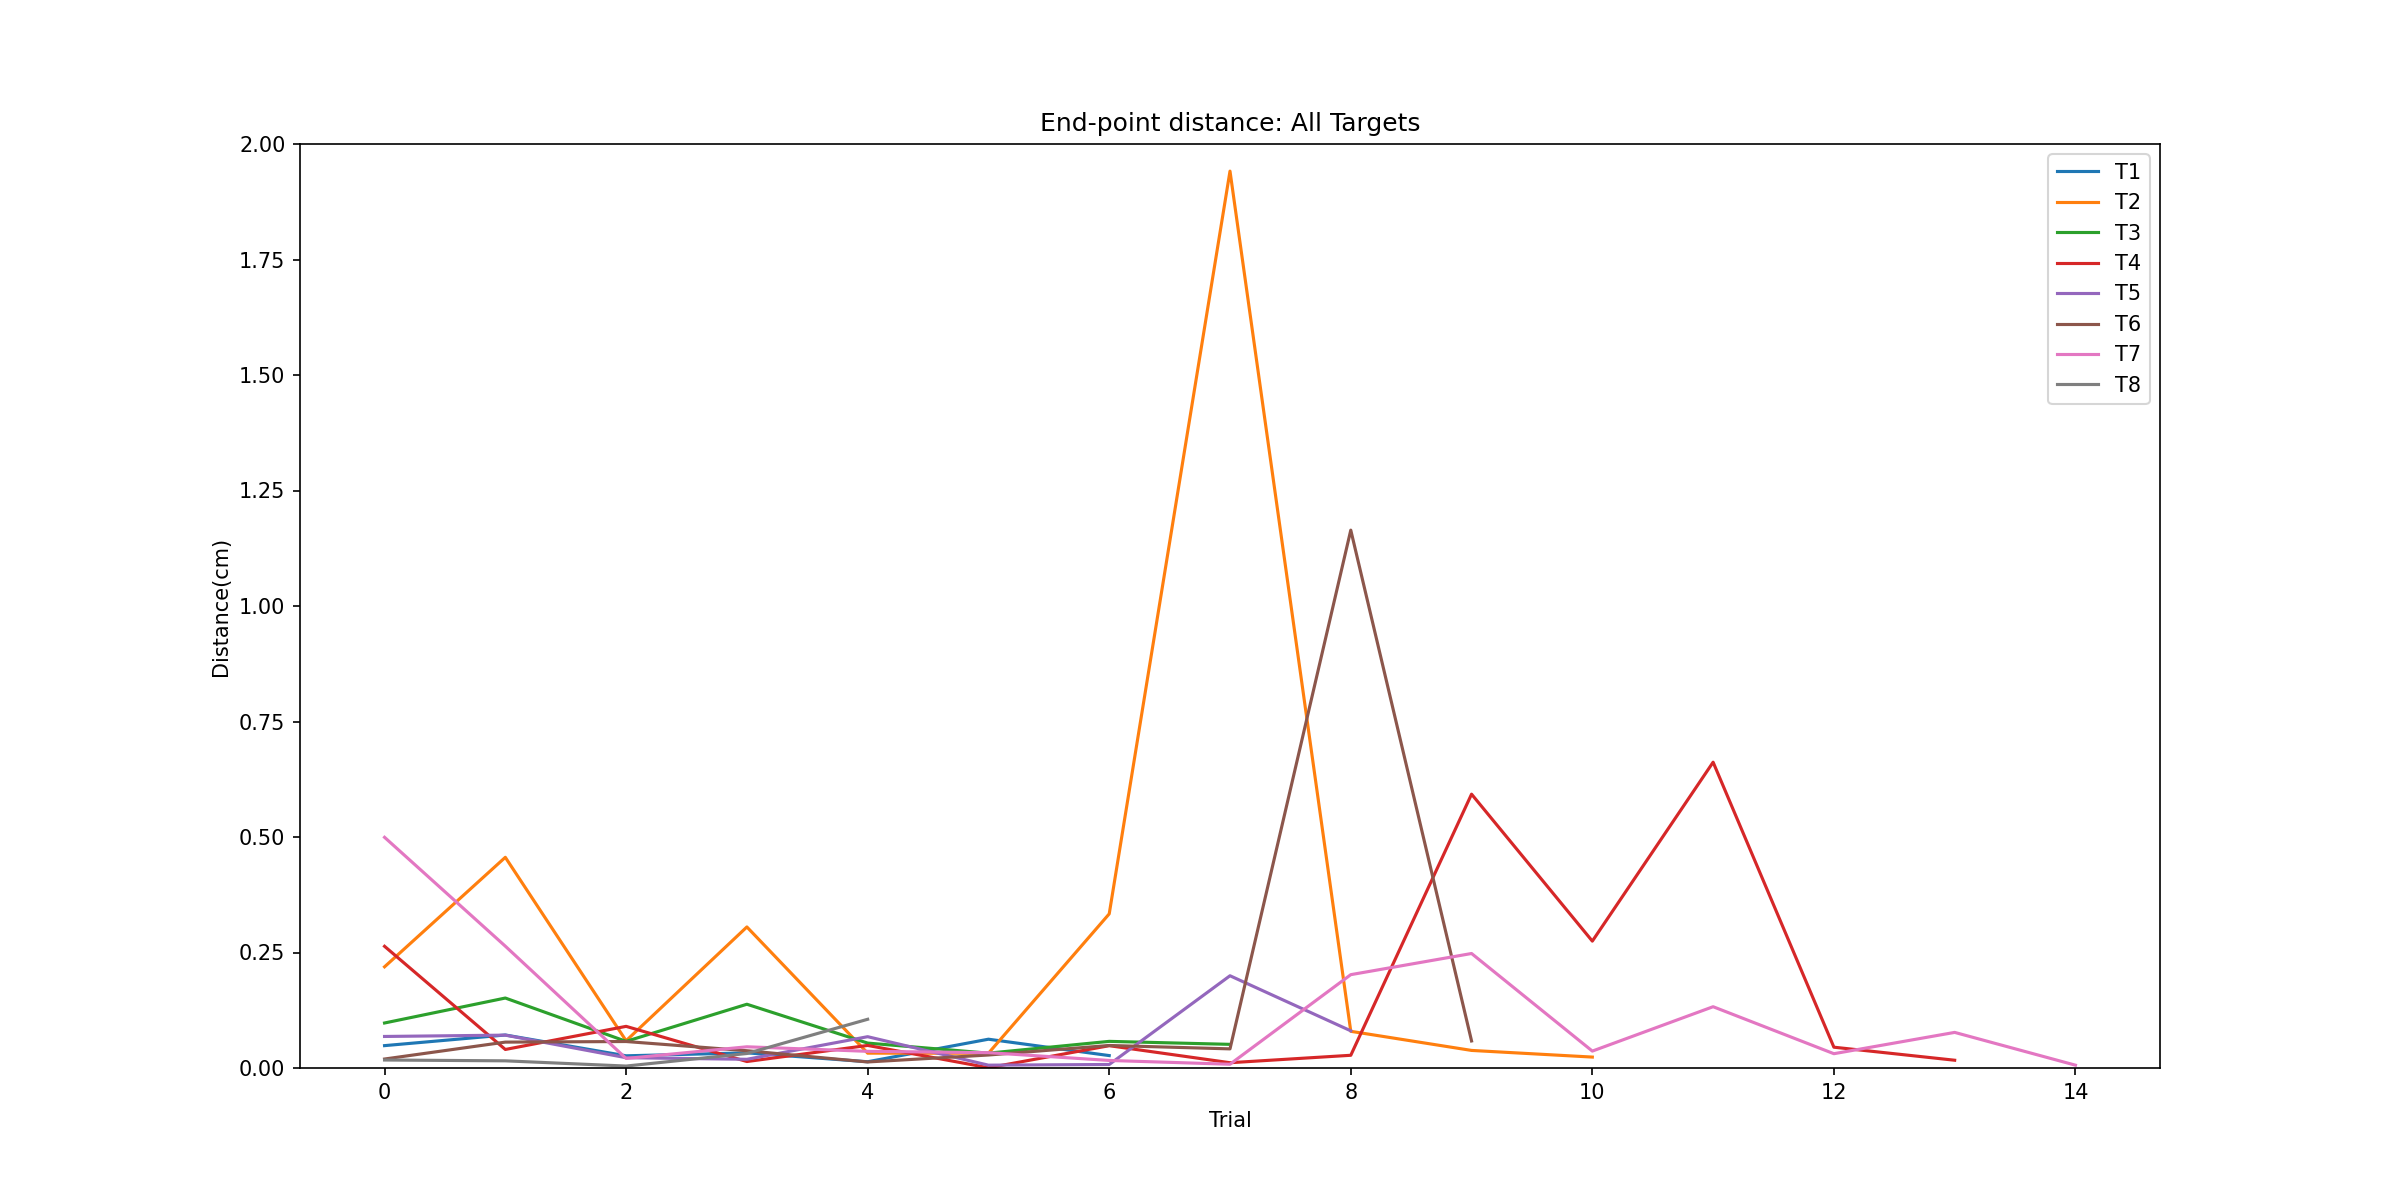
\includegraphics[width=\textwidth]{sujeto3/no_force/evolution_distance}
	
		\end{figure}
	\end{column}
	\end{columns}


\end{frame}


\begin{frame}
	\frametitle{Fase 2: con fuerza}
		\begin{itemize}
		\item Las trayectorias de los sujetos jóvenes son más cortas.
	\end{itemize}
\begin{columns}
	\begin{column}{0.5\textwidth}
		\begin{figure}[t]
			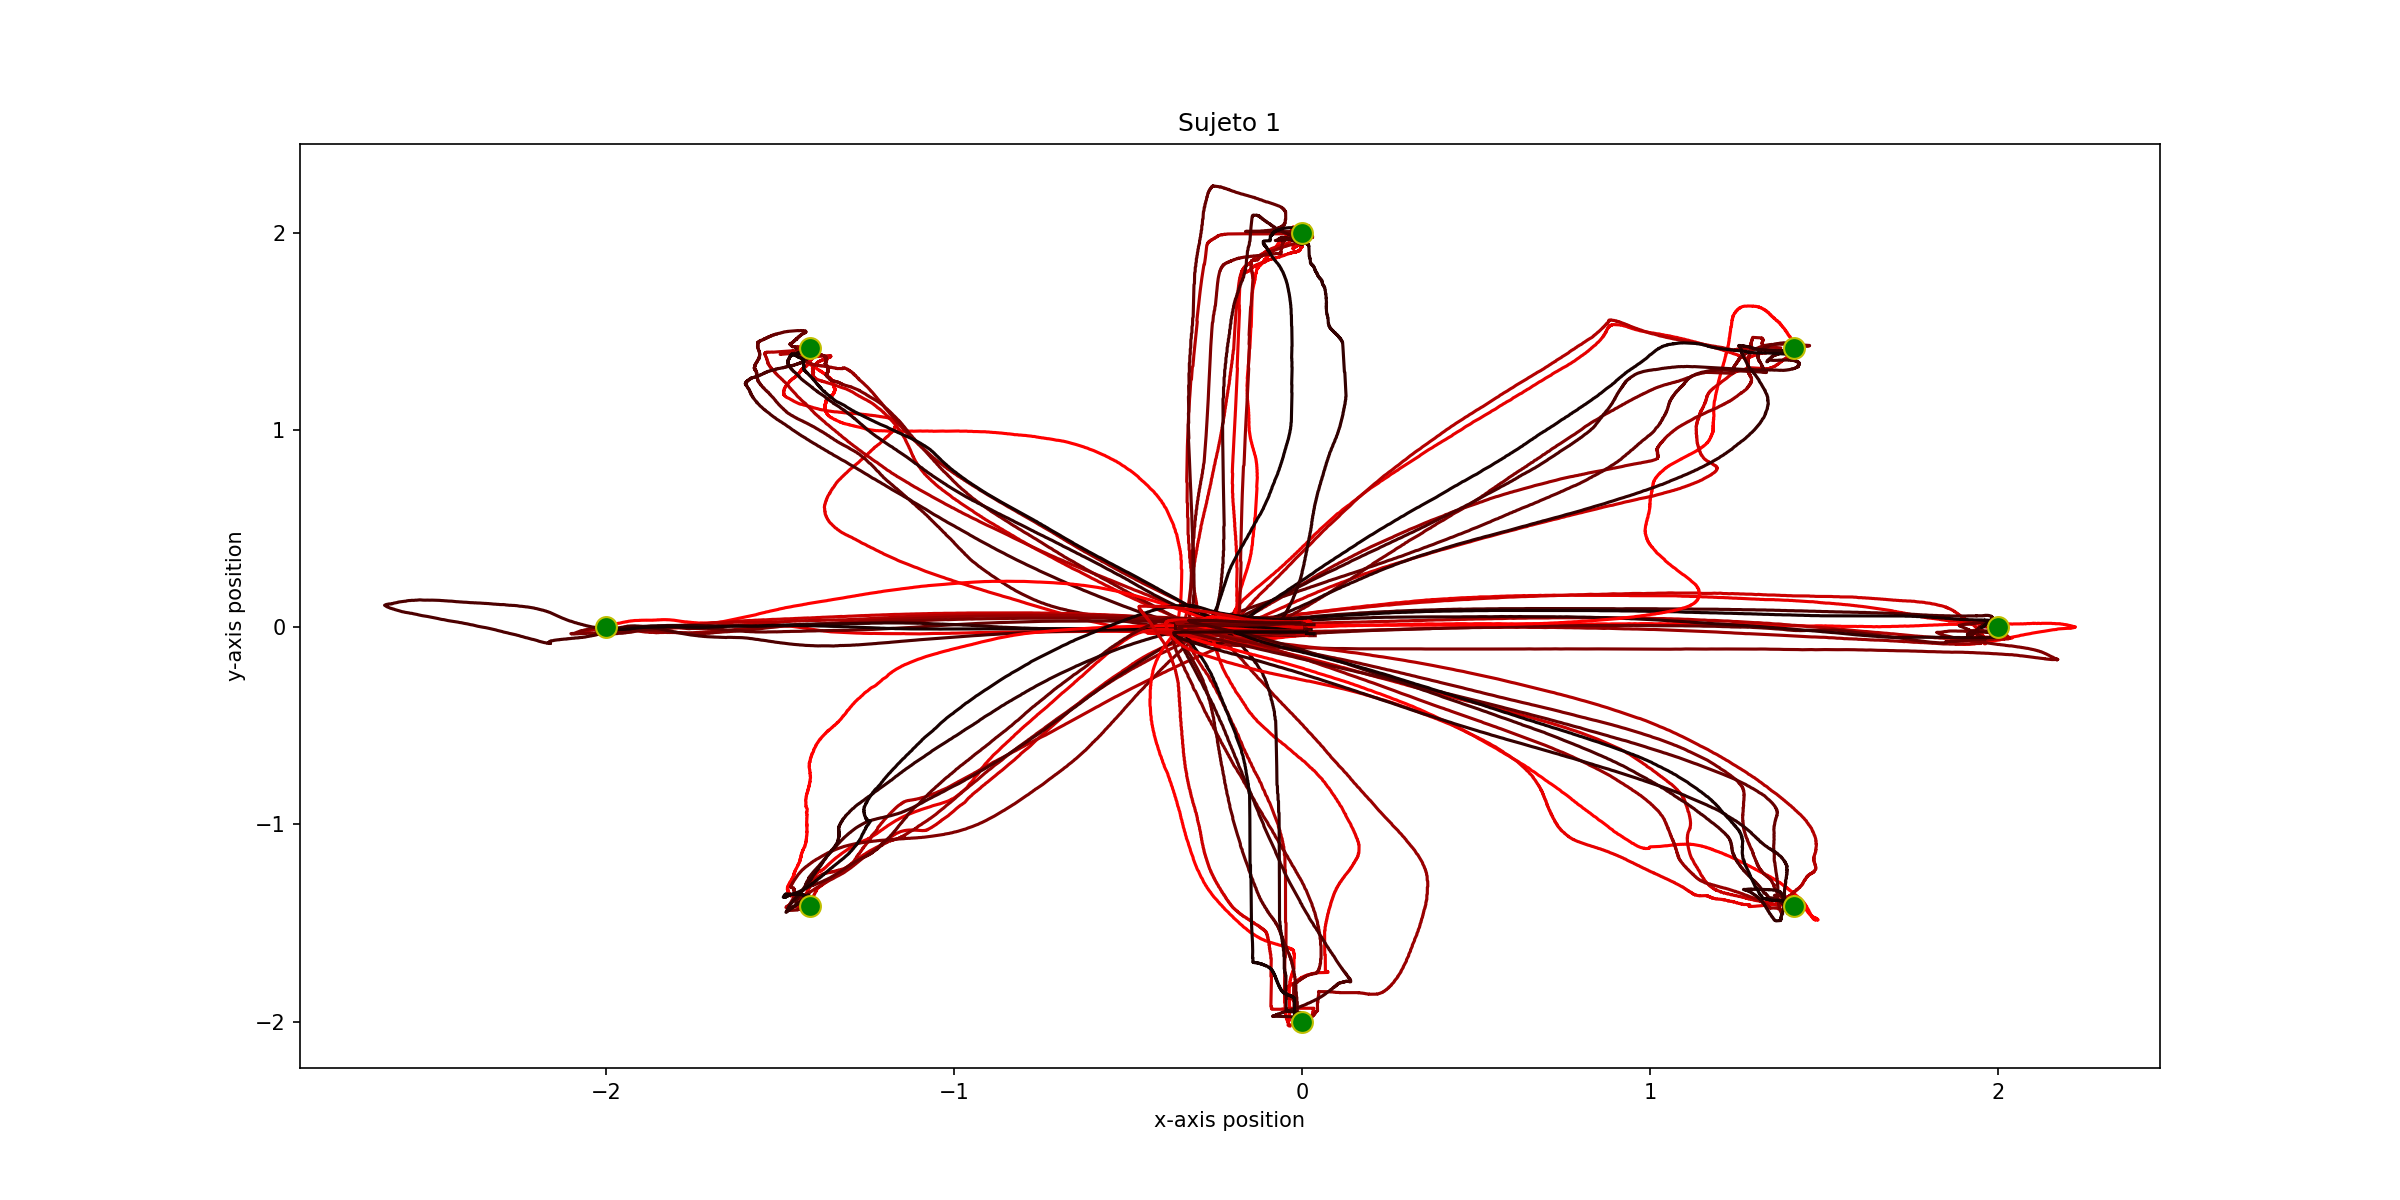
\includegraphics[width=0.88\textwidth]{sujeto1/force/trayectorias}
			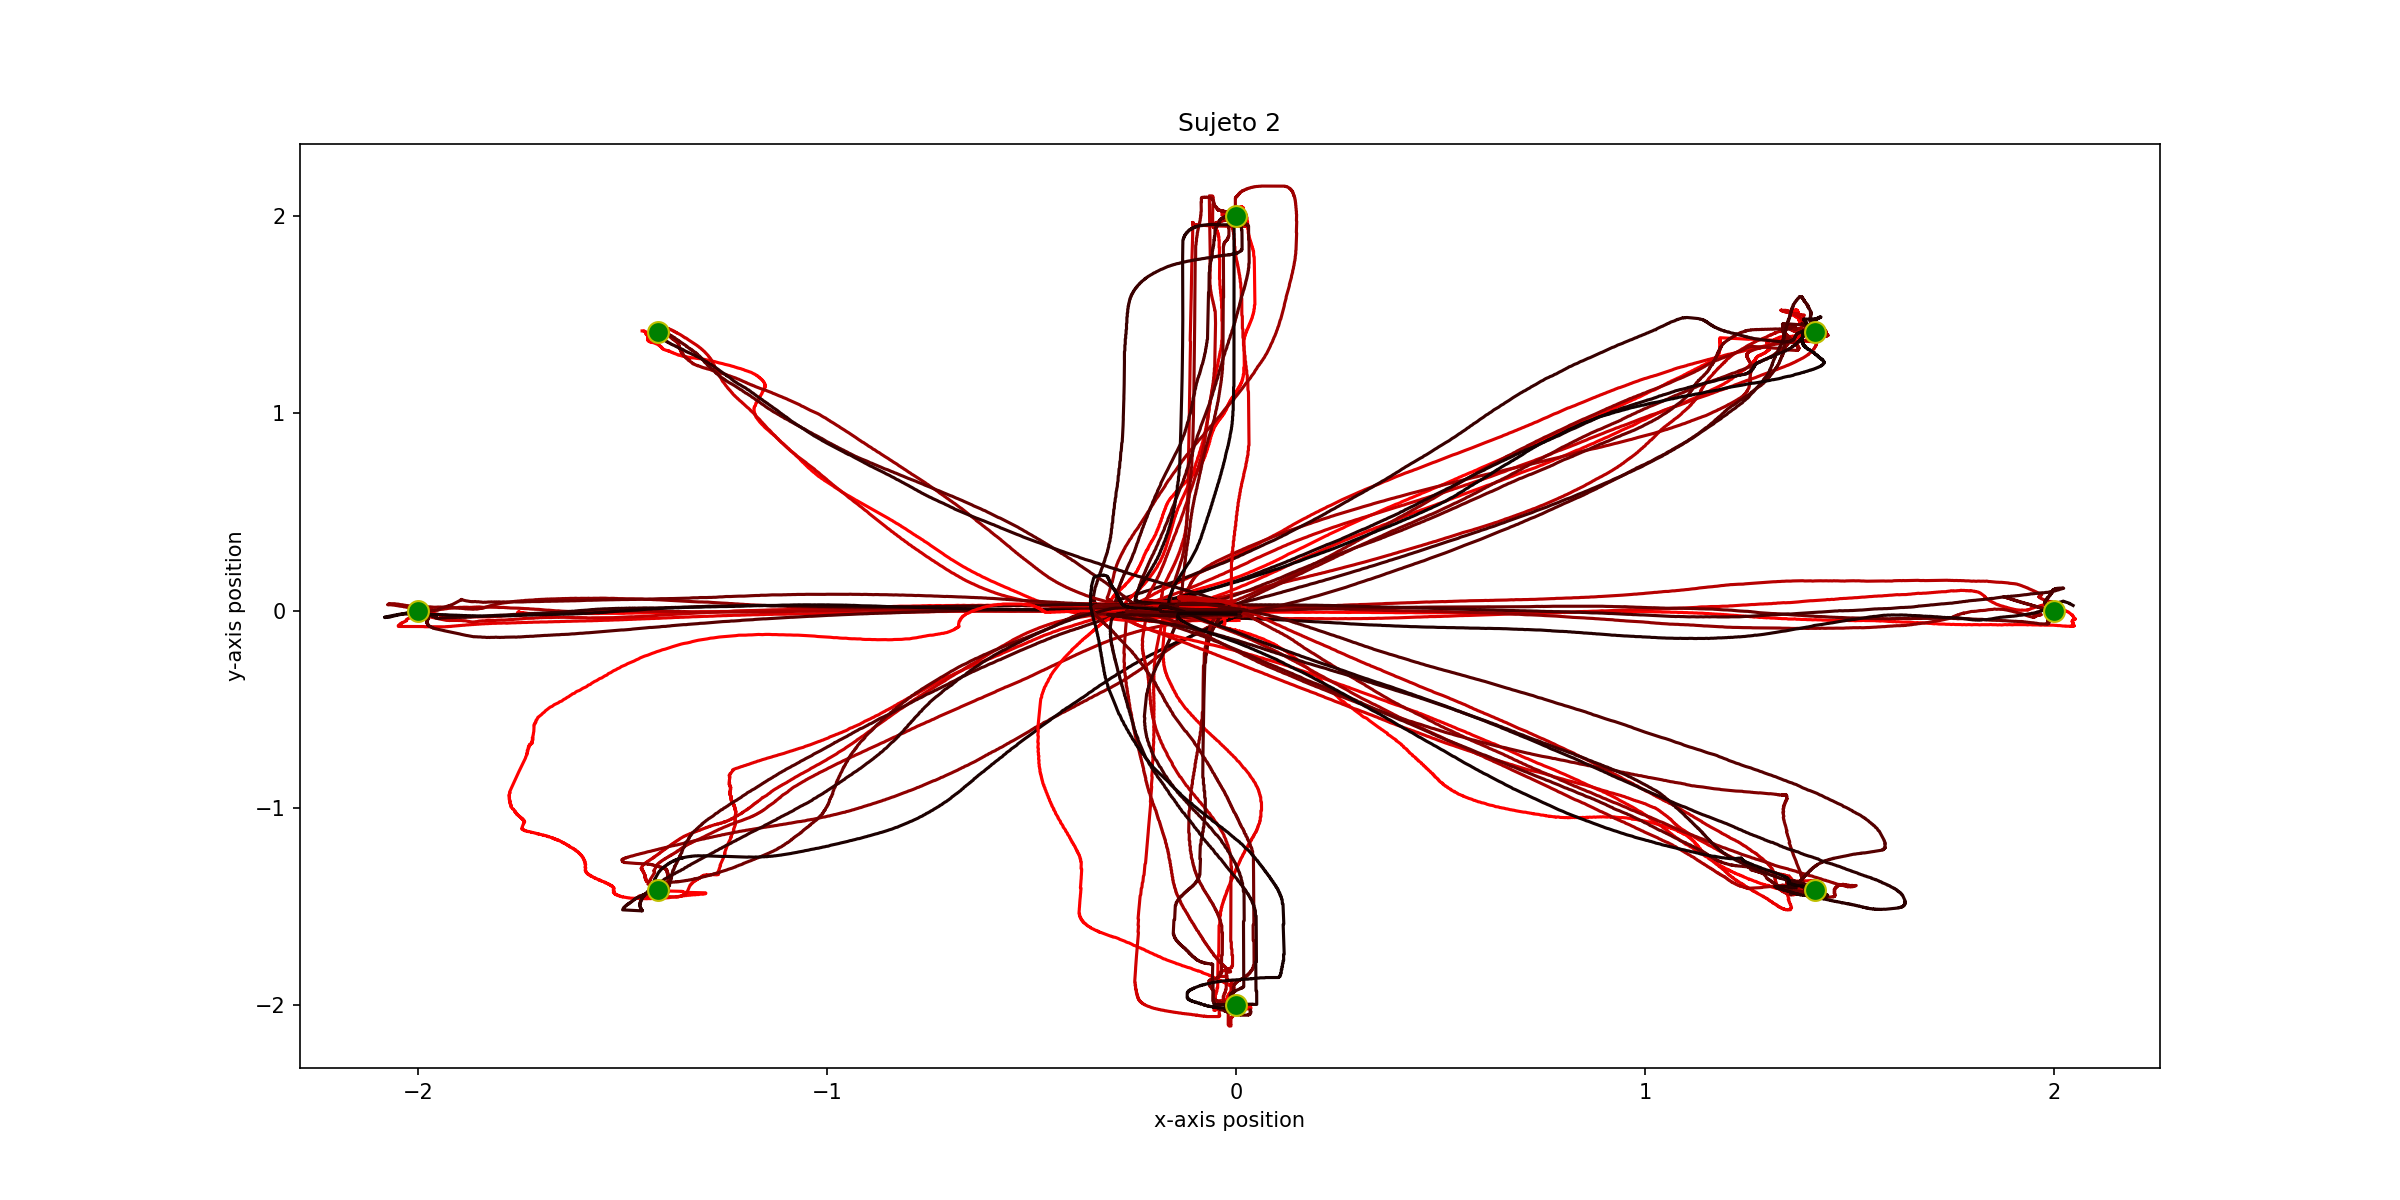
\includegraphics[width=0.88\textwidth]{sujeto2/force/trayectorias}
			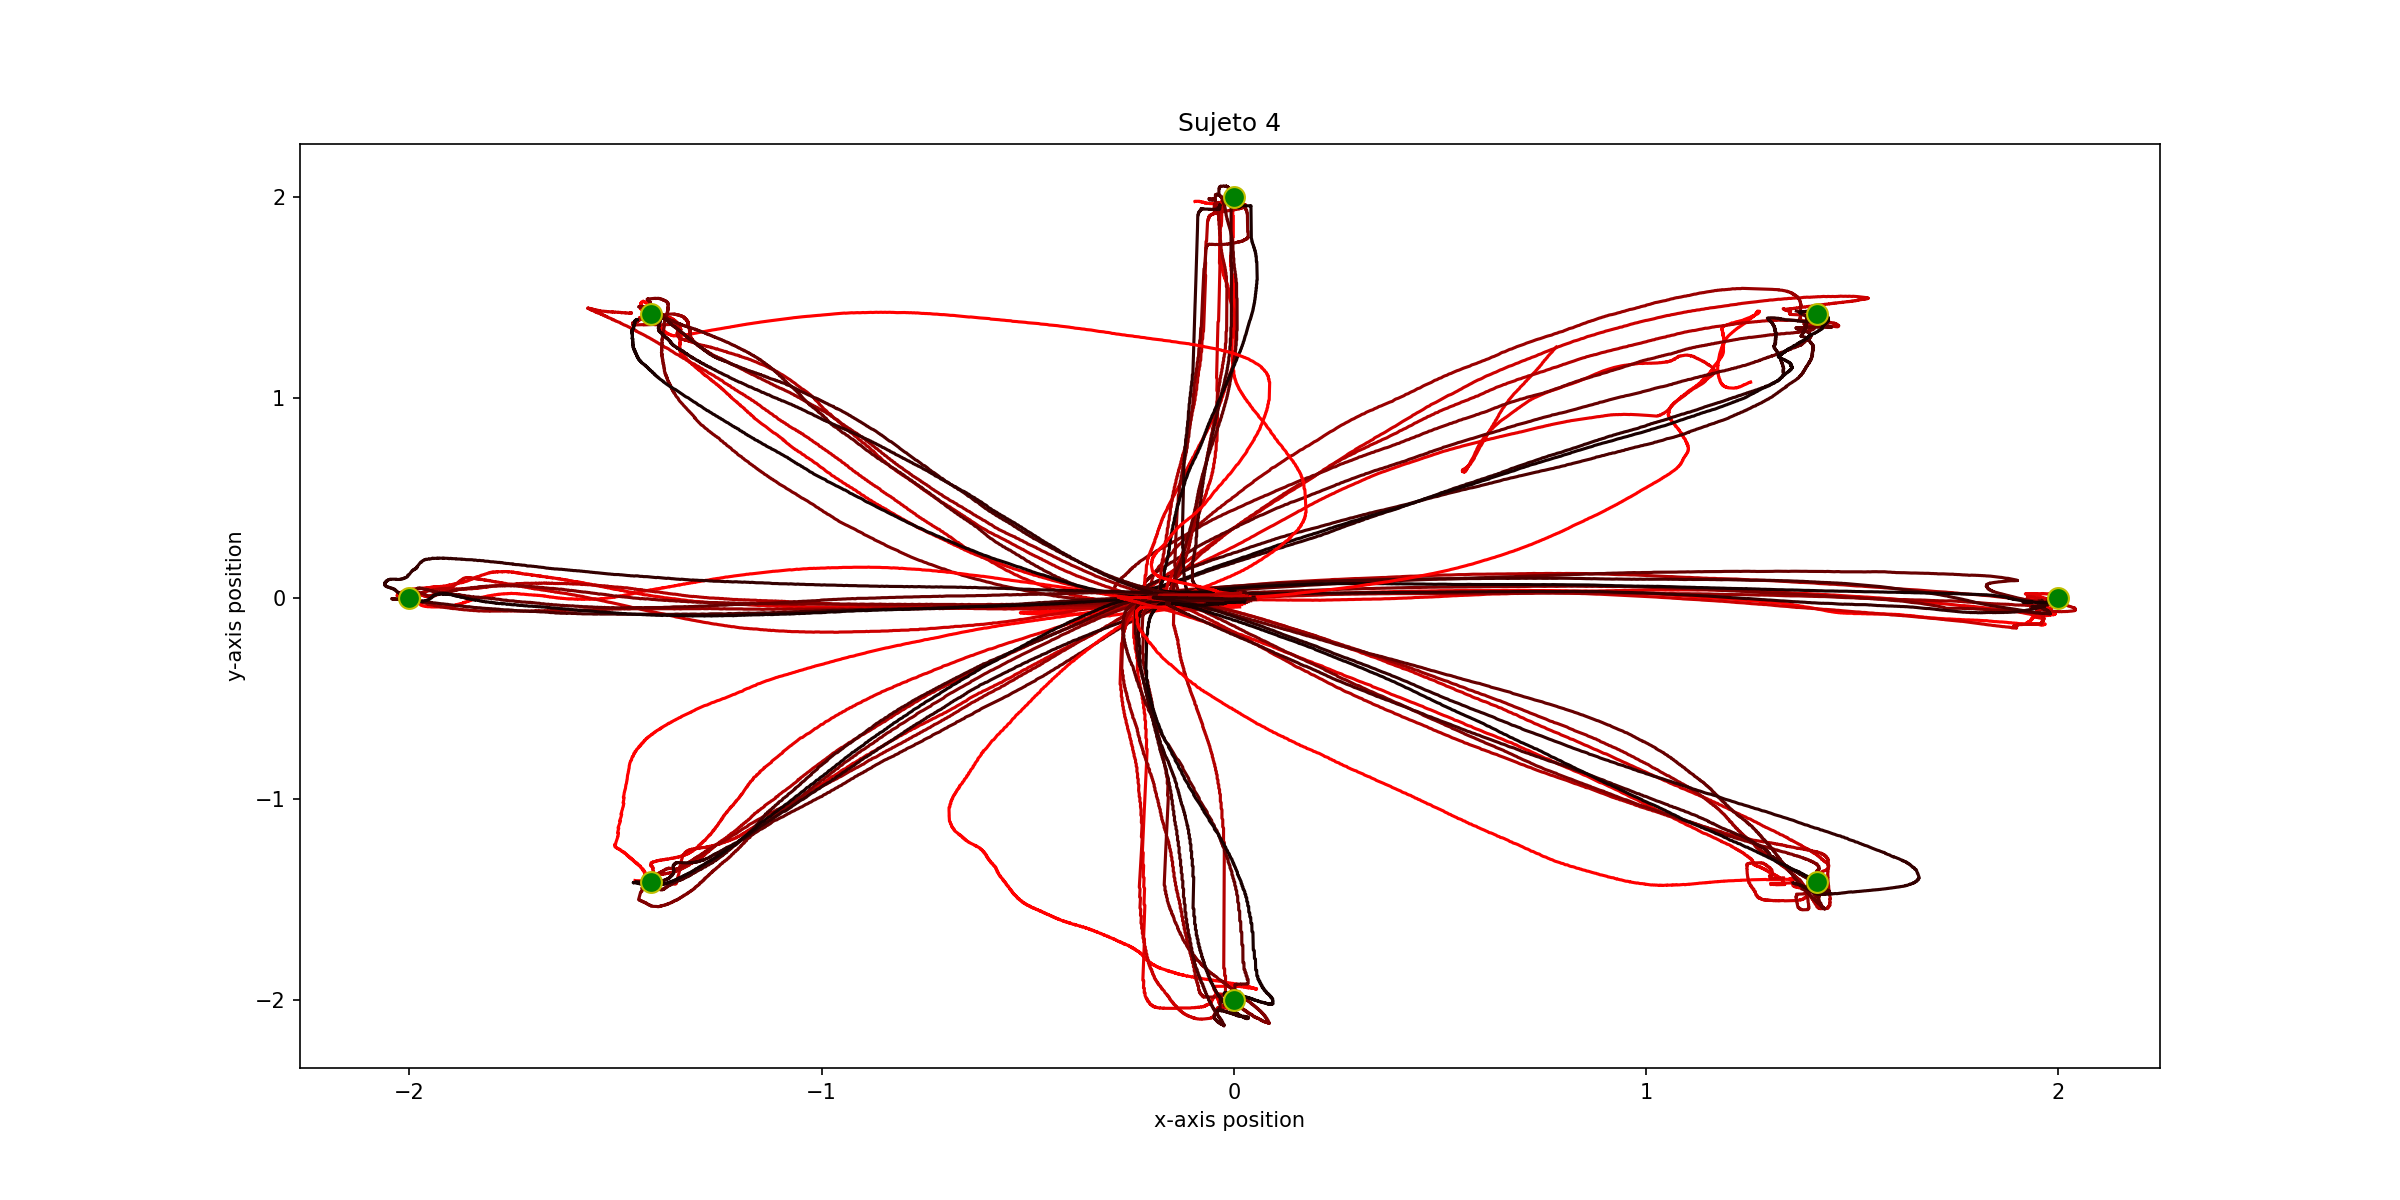
\includegraphics[width=0.88\textwidth]{sujeto4/force/trayectorias}
		\end{figure}
	\end{column}
\begin{column}{0.5\textwidth}
		\begin{figure}
		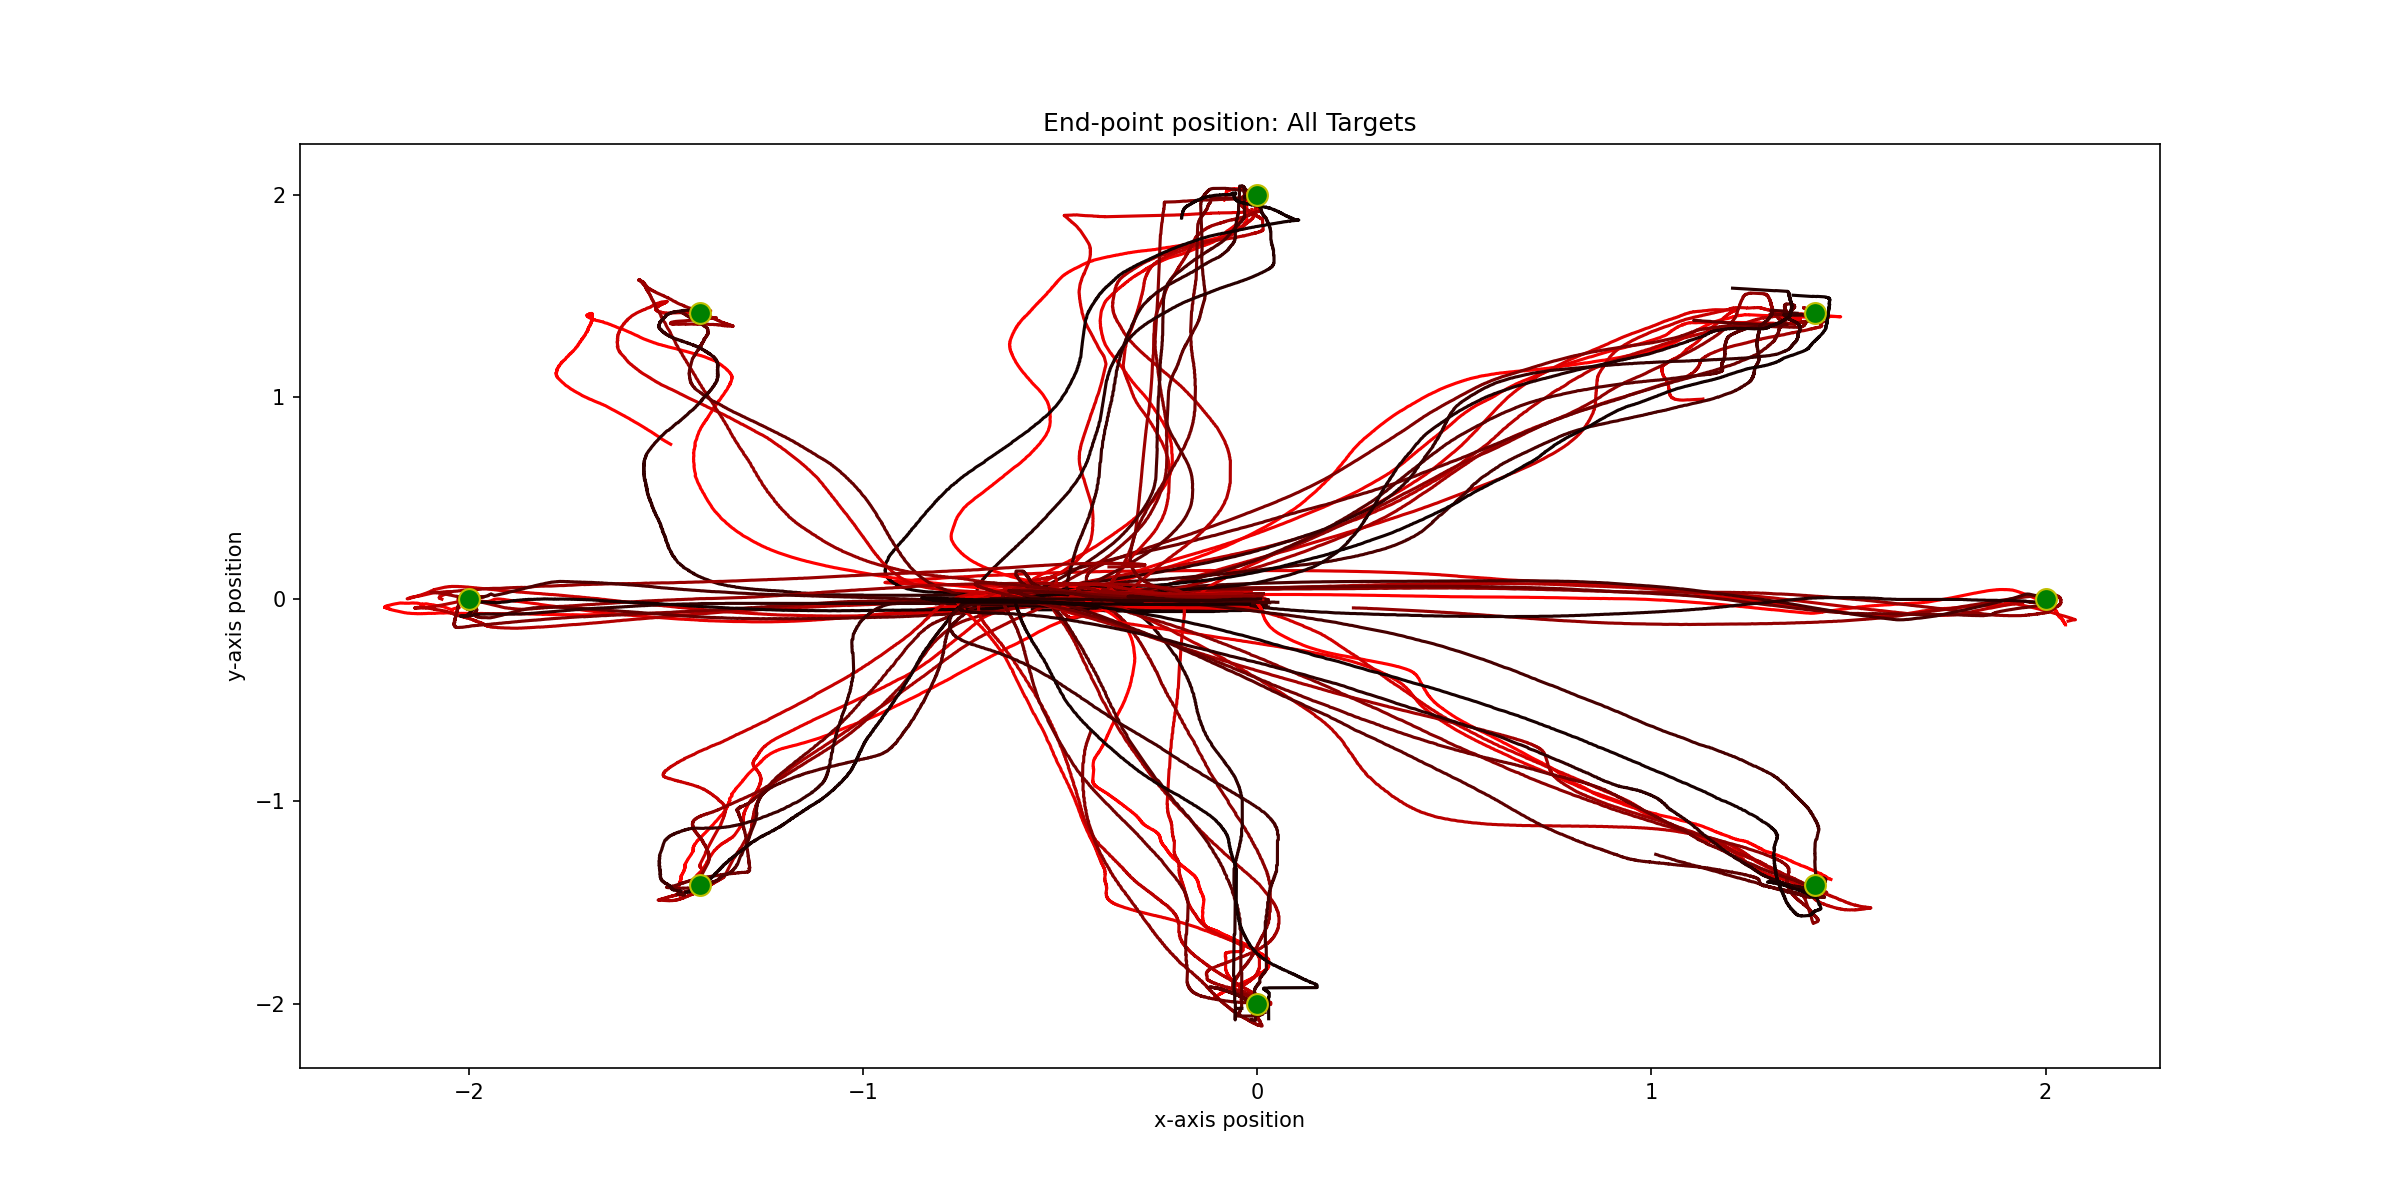
\includegraphics[width=\textwidth]{sujeto3/force/trayectorias}
		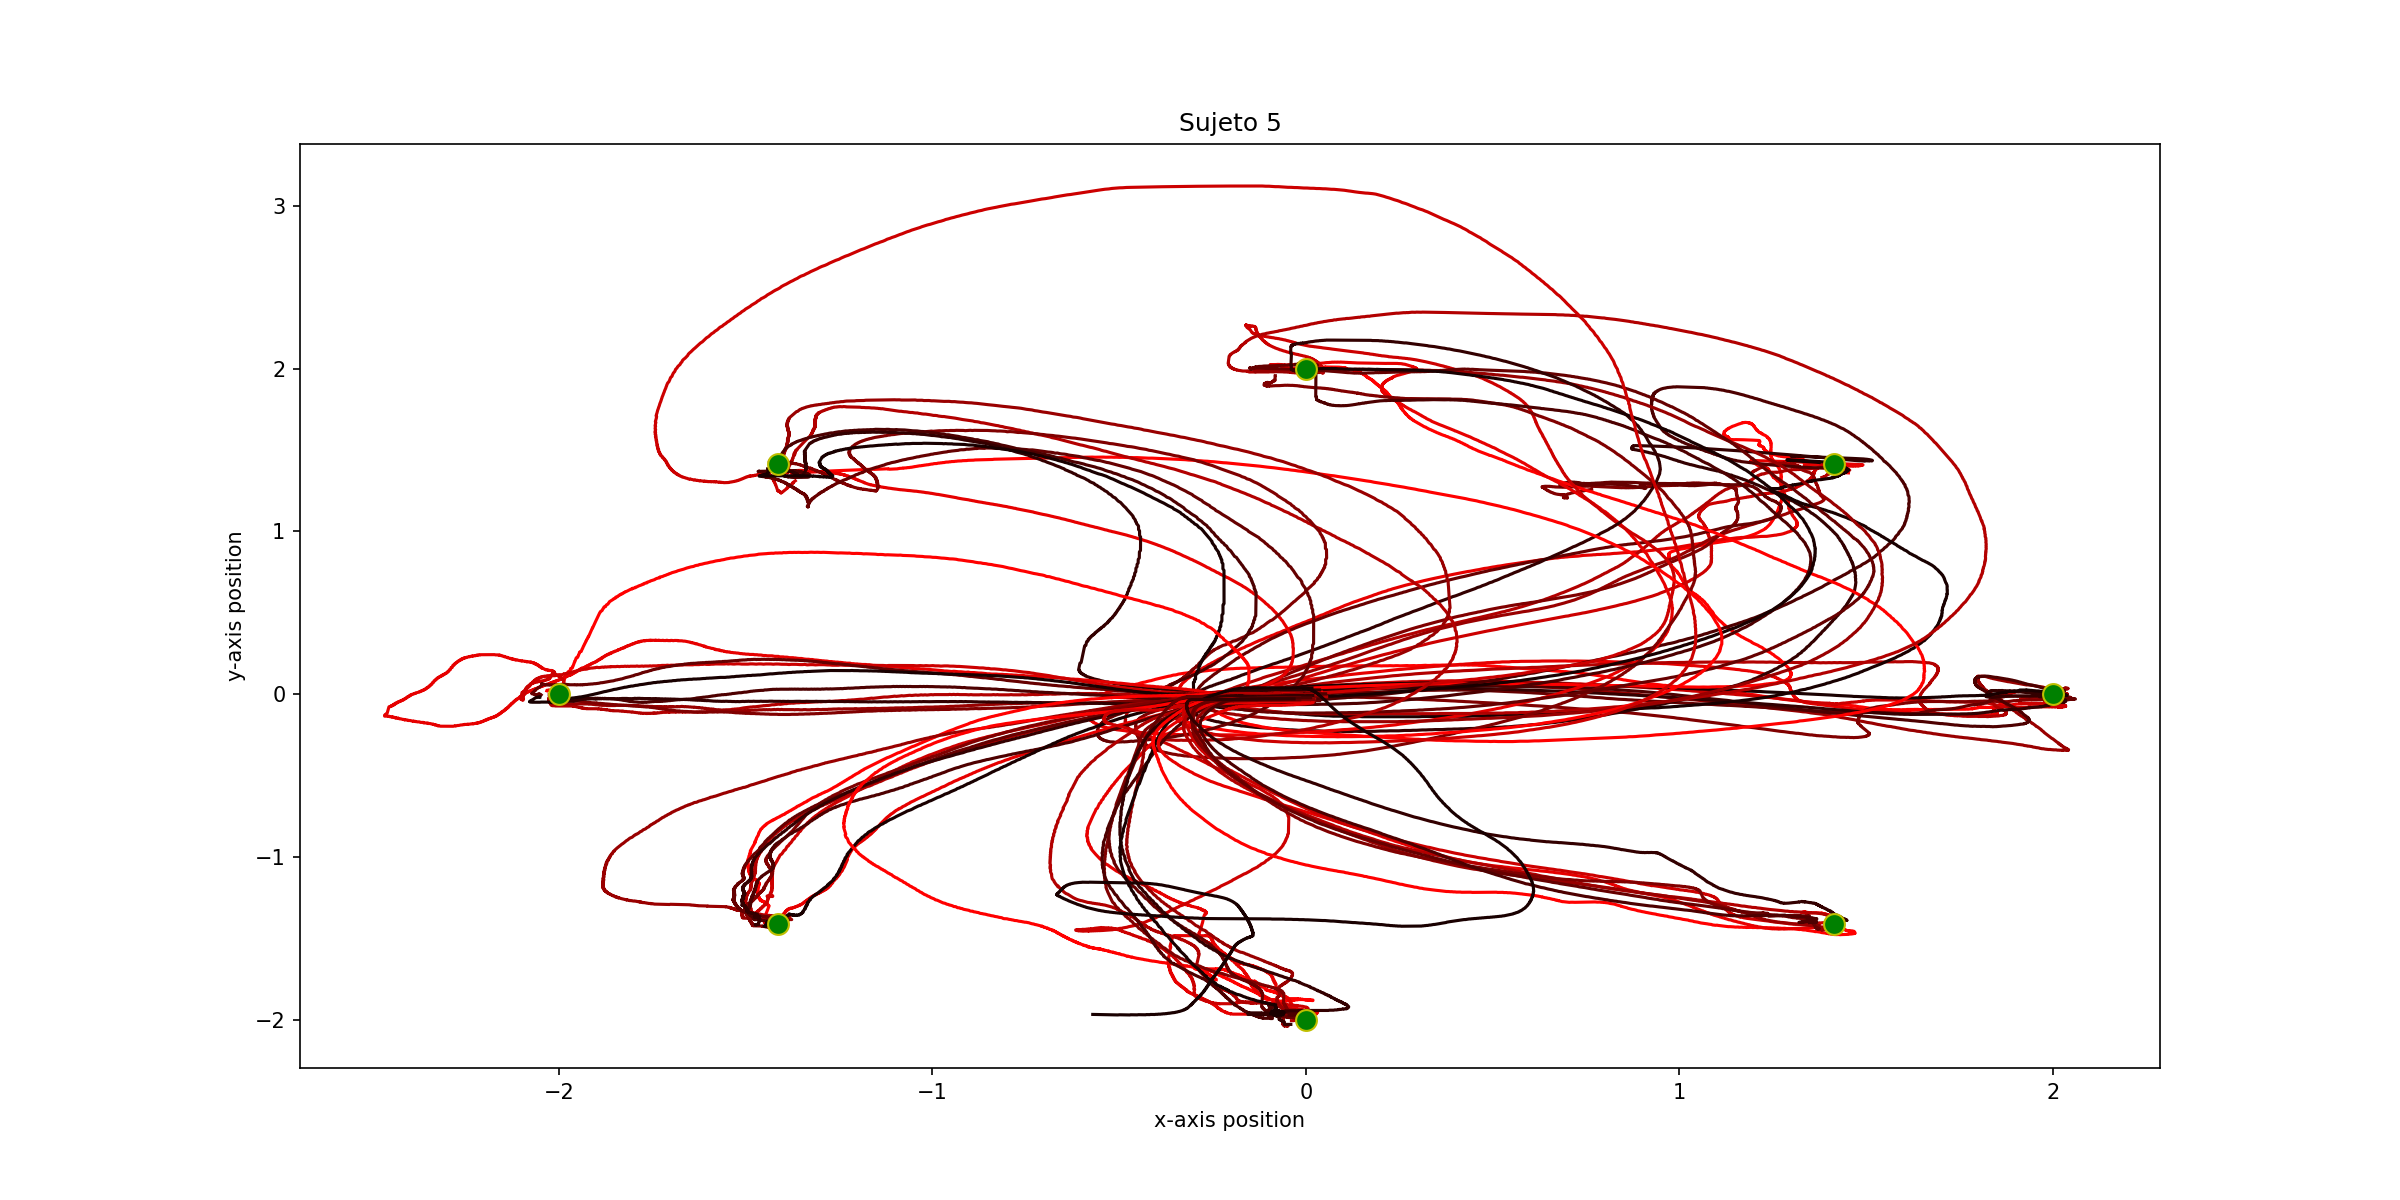
\includegraphics[width=\textwidth]{sujeto5/force/trayectorias}
	\end{figure}
\end{column}
\end{columns}

\end{frame}

\begin{frame}
	\frametitle{Fase 2: con fuerza}
				\begin{itemize}
		\item Los sujetos jóvenes siguen teniendo más precisión.
		\item El sujeto 5 ha extrapolado mejor el movimiento.
	\end{itemize}
	\begin{columns}
		\begin{column}{0.4\textwidth}
			\begin{figure}
				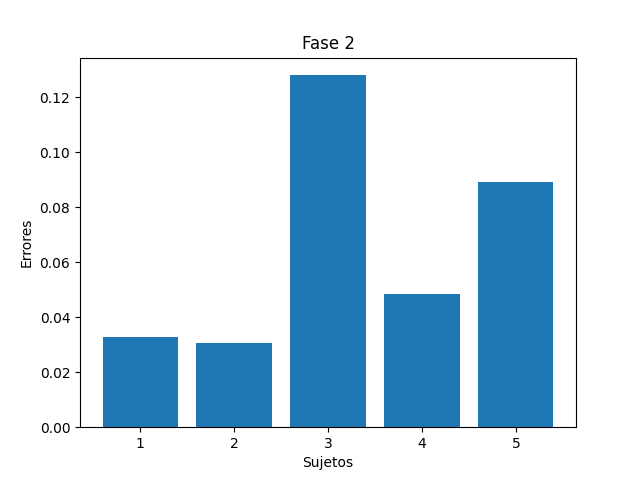
\includegraphics[width=\textwidth]{fase2-errores}
				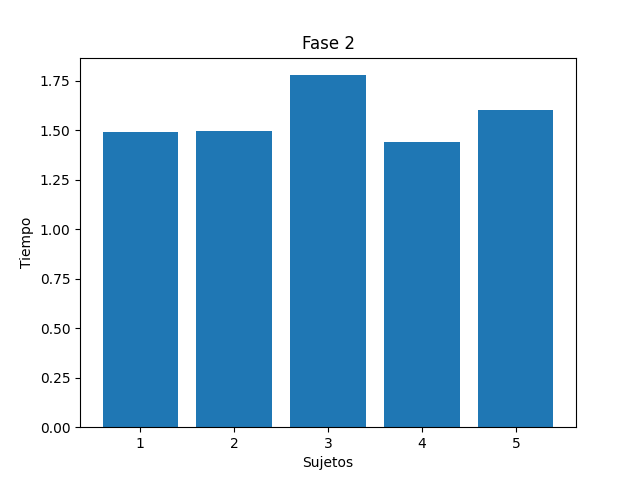
\includegraphics[width=\textwidth]{fase2-time}
			\end{figure}
			
		\end{column}
		\begin{column}{0.6\textwidth}
			\begin{figure}
				\centering
				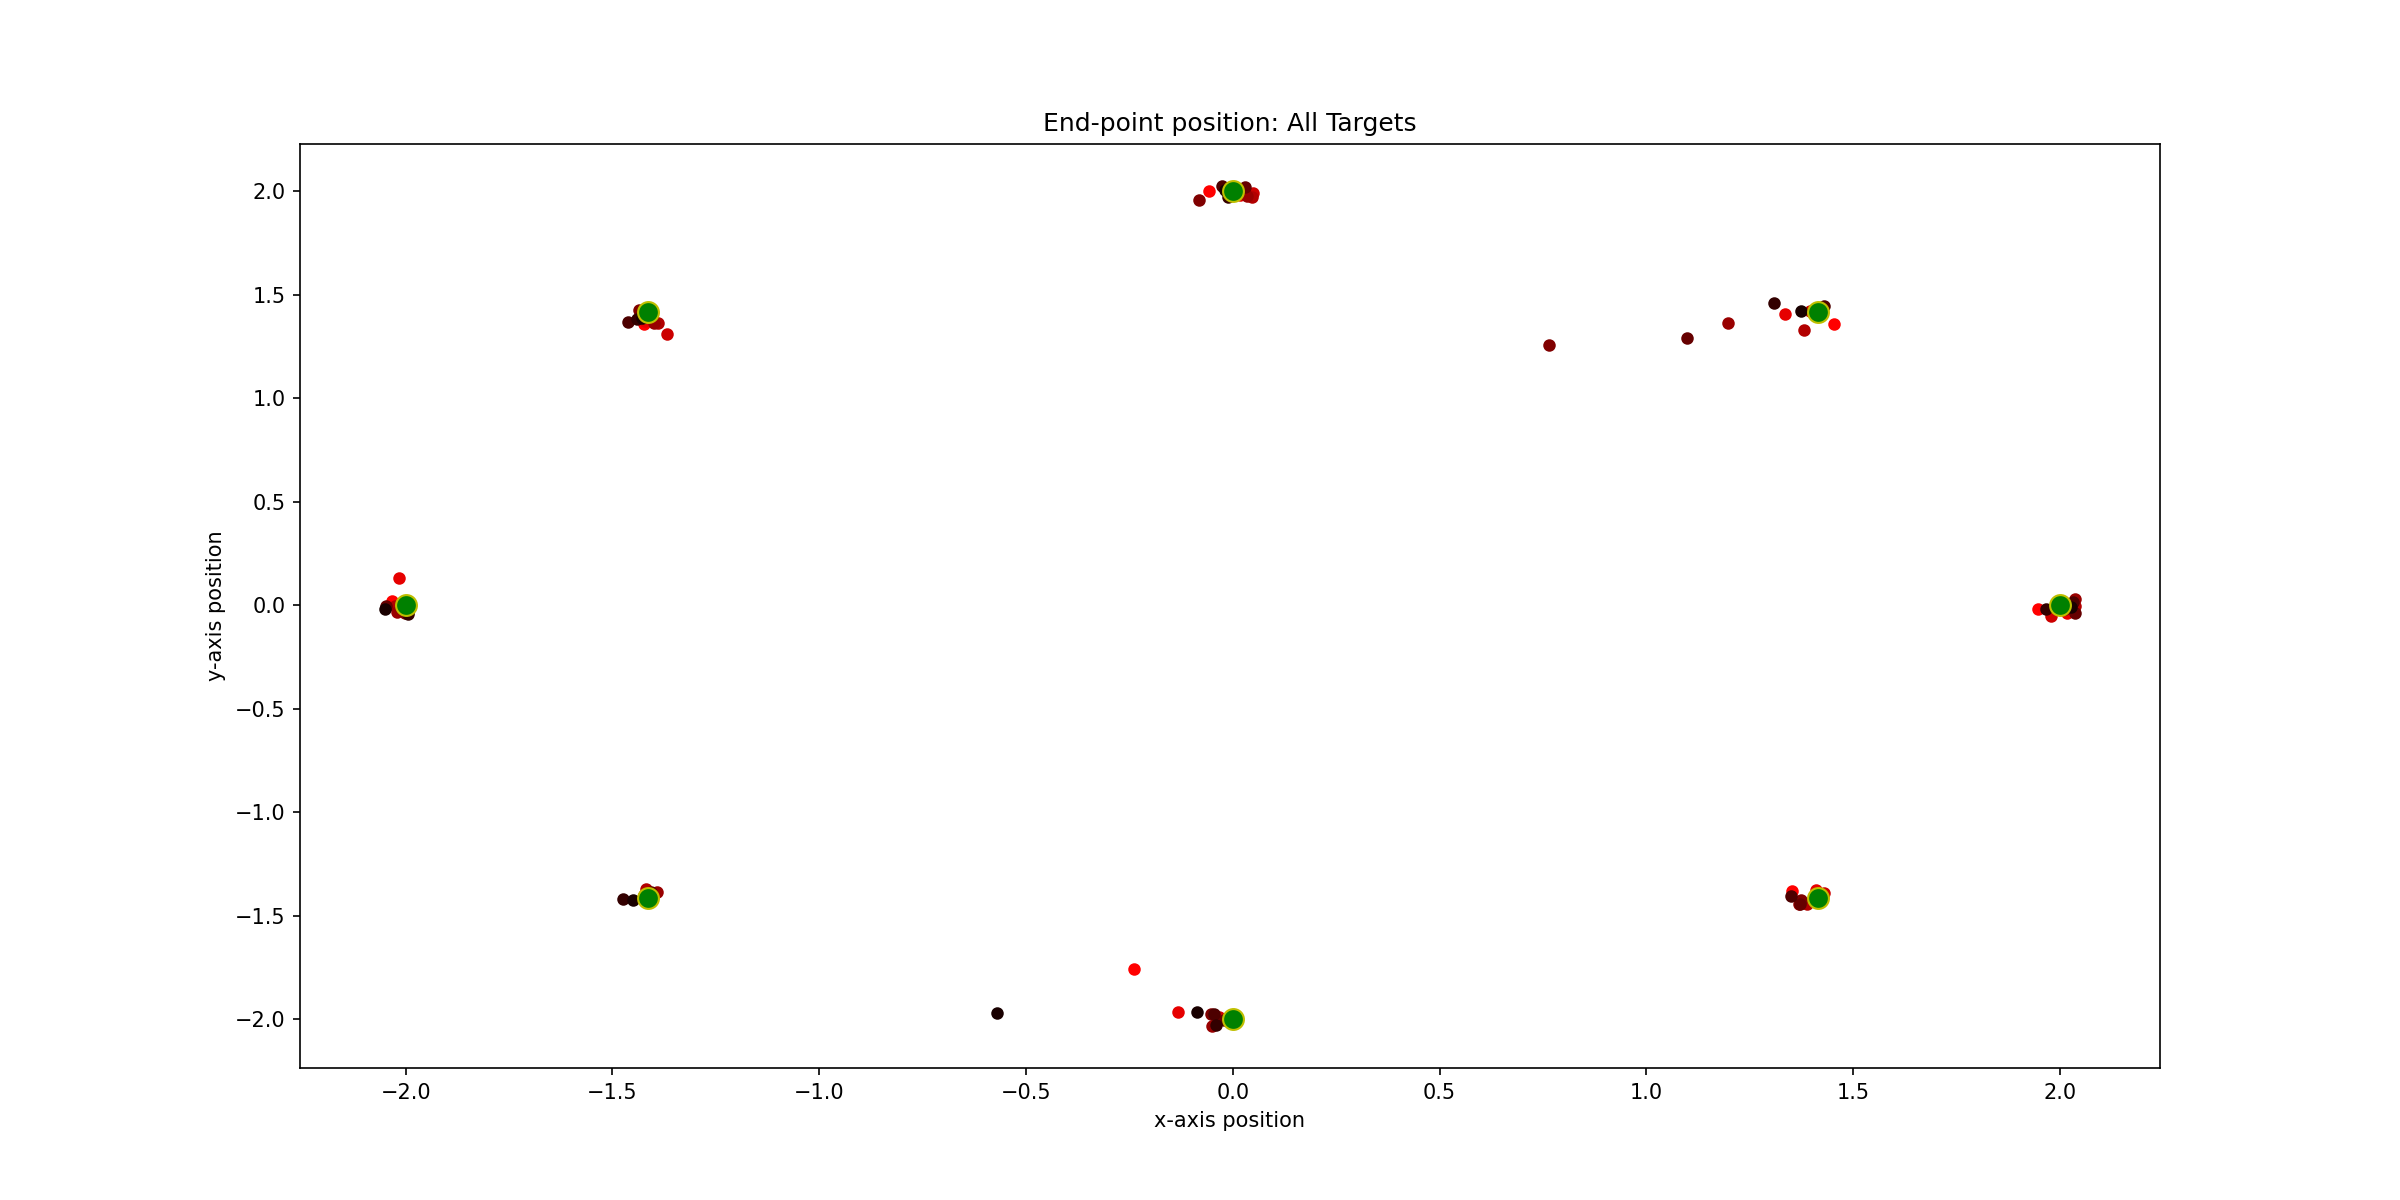
\includegraphics[width=\textwidth]{sujeto5/force/trayectorias_puntos}
				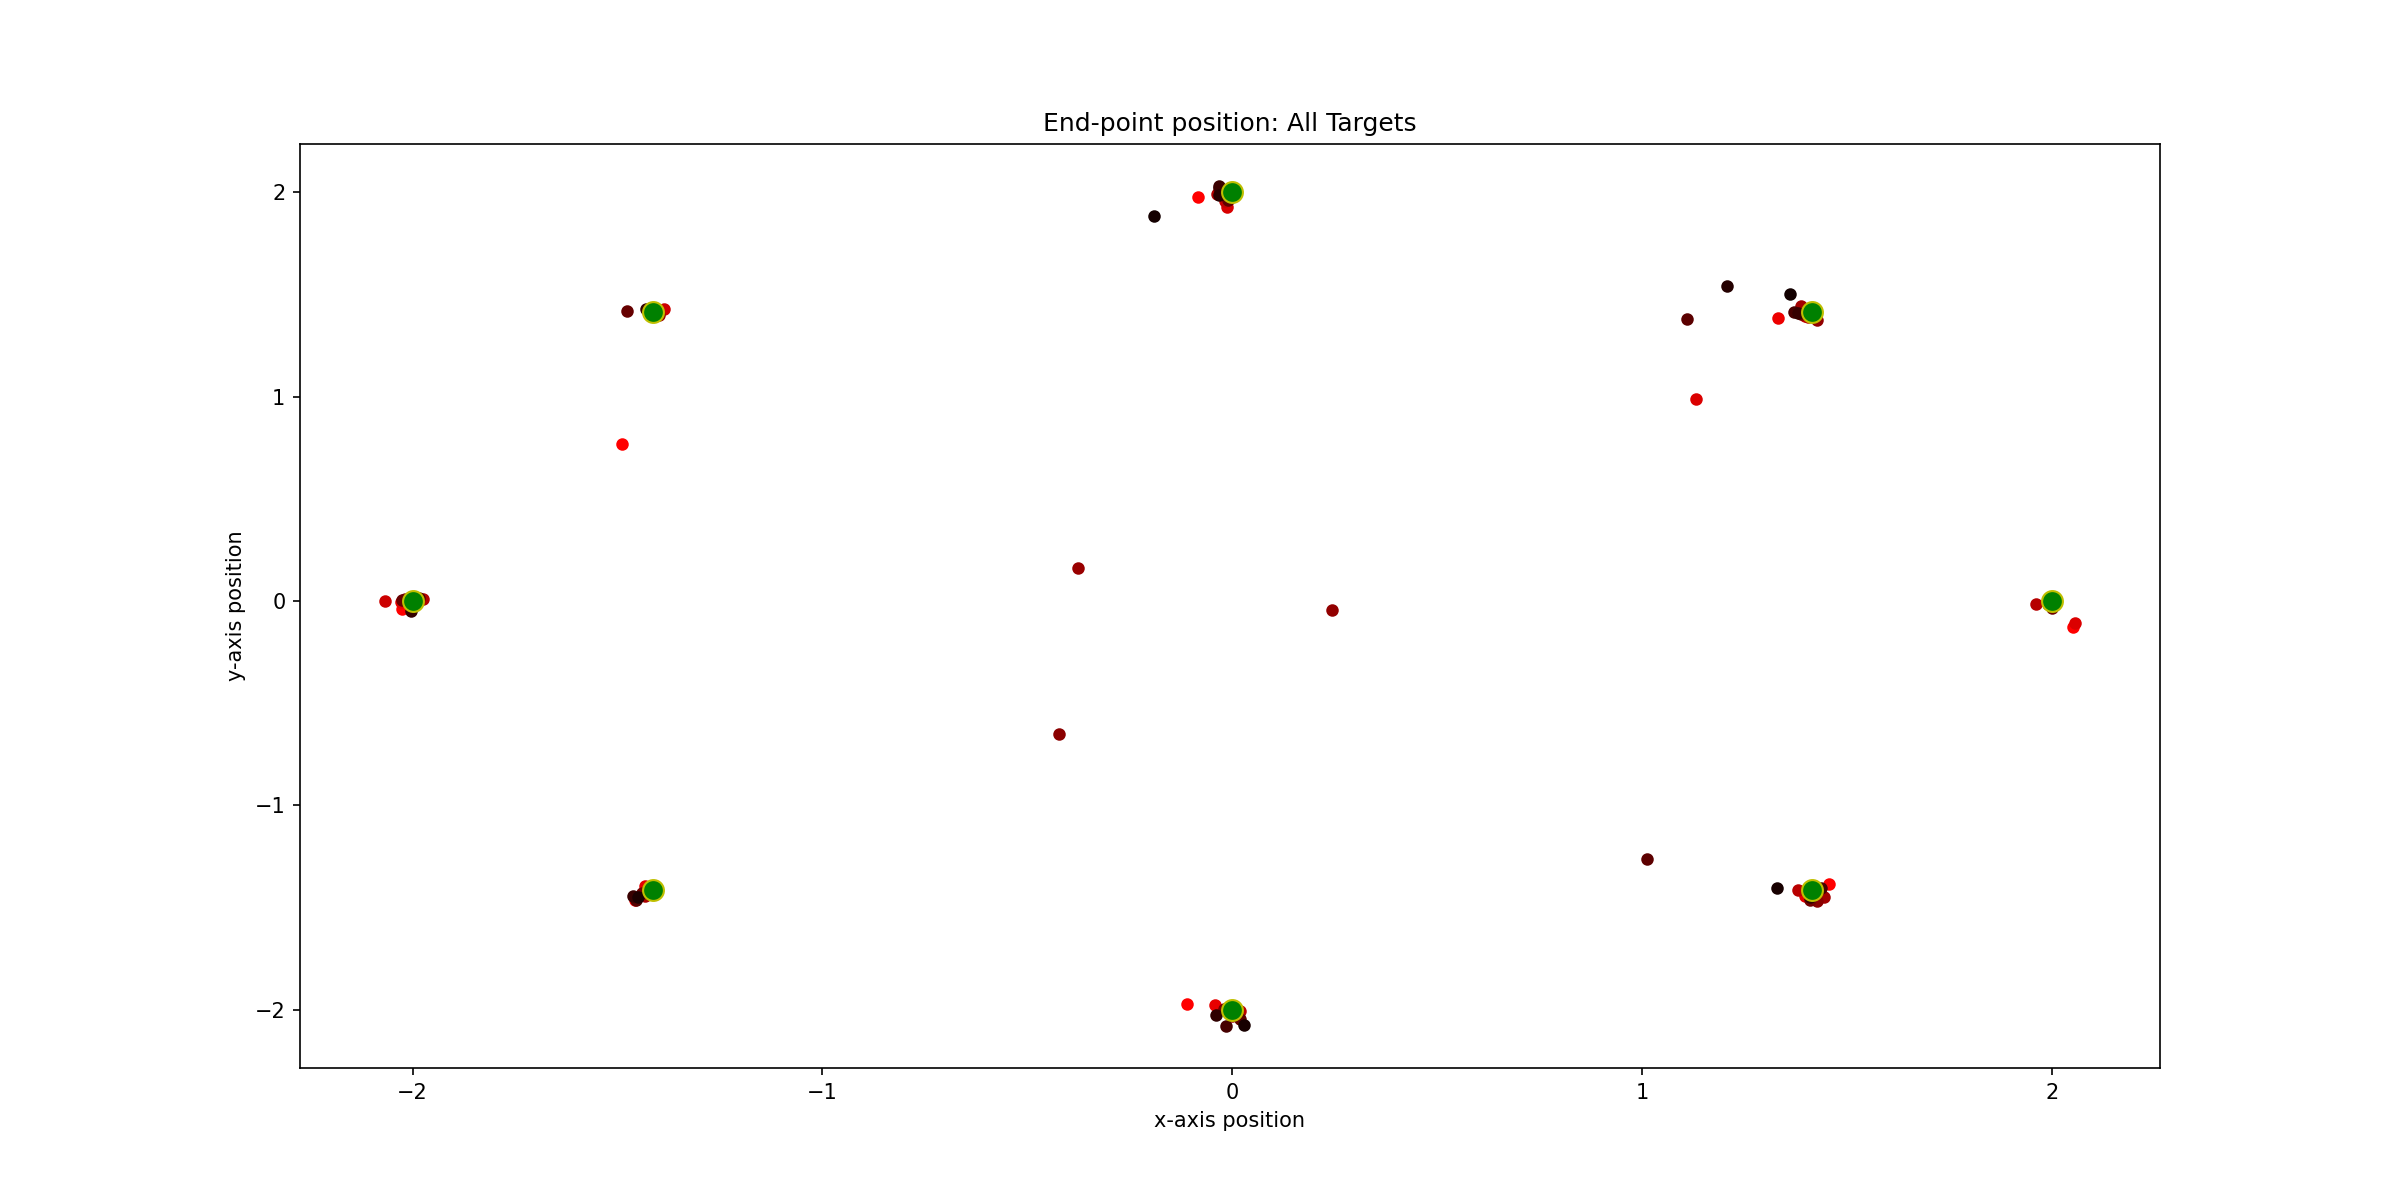
\includegraphics[width=\textwidth]{sujeto3/force/trayectorias_puntos}
				
			\end{figure}
		\end{column}
	\end{columns}

\end{frame}



\begin{frame}
	\frametitle{Fase 3: sin fuerza y sin cursor}
	\begin{figure}
		\centering
		
		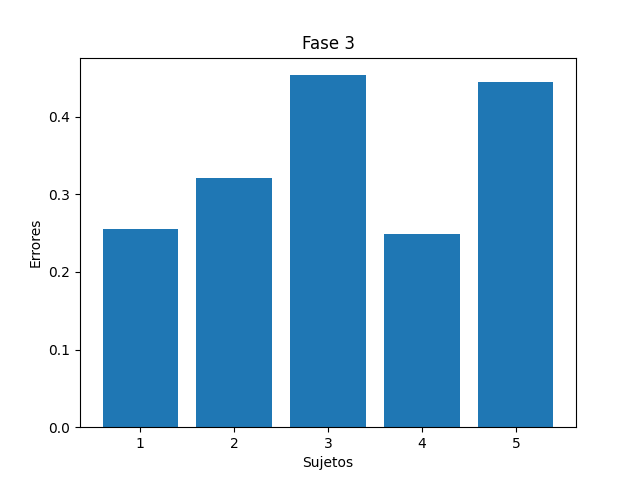
\includegraphics[width=0.45\textwidth]{fase3-errores}
			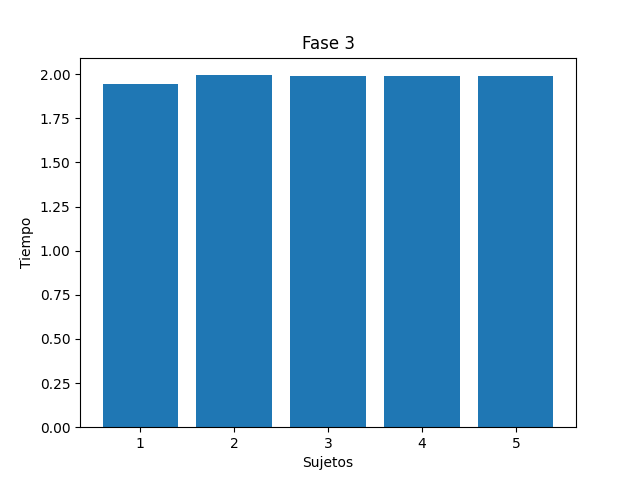
\includegraphics[width=0.45\textwidth]{fase3-time}
	\end{figure}
\begin{itemize}
	\item Los sujetos jóvenes siguen teniendo más precisión.
	\item La precisión de los sujetos mayores es similar.
	\item Casi en ninguna iteración se consigue terminar el movimiento.
\end{itemize}
\end{frame}


\begin{frame}
	\frametitle{Fase 4: con fuerza y sin cursor}
	\begin{figure}
		\centering
		
		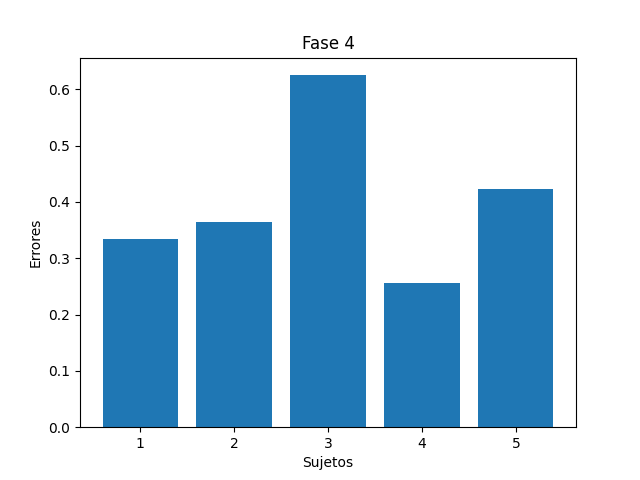
\includegraphics[width=0.45\textwidth]{fase4-errores}
		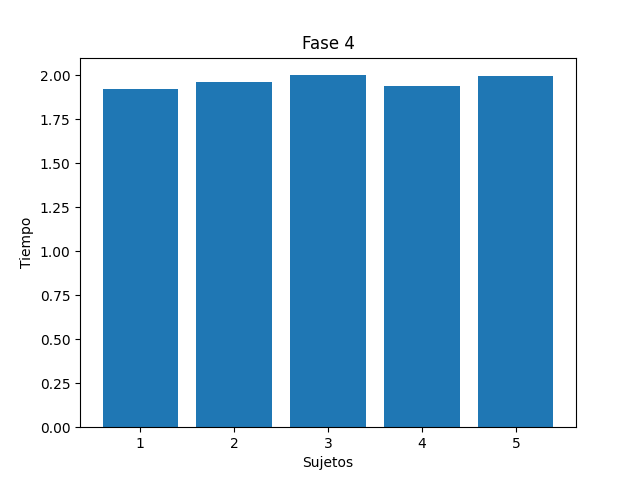
\includegraphics[width=0.45\textwidth]{fase4-time}
	\end{figure}
\begin{itemize}
	\item Los sujetos jóvenes siguen teniendo mejores resultados.
	\item El sujeto 5 mejora considerablemente la precisión.
\end{itemize}
\end{frame}


\section{Conclusiones}
\begin{frame}
	\frametitle{Conclusiones}
	Todos los objetivos cumplidos:
	\begin{itemize}
		\item Desarrollo de una aplicación con un dispositivo háptico.
		\item Estudiar si los datos recogidos son útiles, y cómo interpretarlos.
		\item Desarrollo de un experimento científico:
		\begin{itemize}
			\item Planificación
			\item Plataforma de experimentación
			\item Obtención y análisis de resultados
		\end{itemize}
	\end{itemize}

\end{frame}
\begin{frame}
	\frametitle{Conclusiones adicionales y vías futuras}
	Conclusiones adicionales que podemos obtener:
	\begin{itemize}
		\item Diferencia de resultados entre las personas jóvenes y las personas mayores.
		\item En la mayoría de los sujetos la fuerza afecta más a la precisión cuando se oculta el cursor.
		\item La aparición en orden (o no) de los puntos afecta más a las personas mayores.
	\end{itemize}
	Aplicaciones futuras:
	\begin{itemize}
		\item Estudio con pacientes con daños cerebrales. 
	\end{itemize}
\end{frame}


\end{document}
